% В этом файле следует писать текст работы, разбивая его на
% разделы (section), подразделы (subsection) и, если нужно,
% главы (chapter).

% Предварительно следует указать необходимую информацию
% в файле SETUP.tex

%% В этот файл не предполагается вносить изменения

% В этом файле следует указать информацию о себе
% и выполняемой работе.

\documentclass [fontsize=14pt, paper=a4, pagesize, DIV=calc]%
{scrreprt}
% ВНИМАНИЕ! Для использования глав поменять
% scrartcl на scrreprt

% Здесь ничего не менять
\usepackage [T2A] {fontenc}   % Кириллица в PDF файле
\usepackage [utf8] {inputenc} % Кодировка текста: utf-8
\usepackage [russian] {babel} % Переносы, лигатуры

%%%%%%%%%%%%%%%%%%%%%%%%%%%%%%%%%%%%%%%%%%%%%%%%%%%%%%%%%%%%%%%%%%%%%%%%
% Создание макроса управления элементами, специфичными
% для вида работы (курс., бак., маг.)
% Здесь ничего не менять:
\usepackage{ifthen}
\newcounter{worktype}
\newcommand{\typeOfWork}[1]
{
	\setcounter{worktype}{#1}
}

% ВНИМАНИЕ!
% Укажите тип работы: 0 - курсовая, 1 - бак., 2 - маг.,
% 3 - бакалаврская с главами.
\typeOfWork{2}
% Считается, что курсовая и бак. бьются на разделы (section) и
% подразделы (subsection), а маг. — на главы (chapter), разделы и
%  подразделы. Если хочется,
% чтобы бак. была с главами (например, если она большая),
% надо выбрать опцию 3.

% Если при выборе 2 или 3 вы забудете поменять класс
% документа на scrreprt (см. выше, в самом начале),
% то получите ошибку:
% ./aux/appearance.tex:52: Package scrbase Error: unknown option ` chapterprefix=

%%%%%%%%%%%%%%%%%%%%%%%%%%%%%%%%%%%%%%%%%%%%%%%%%%%%%%%%%%%%%%%%%%%%%%%%
% Информация об авторе и работе для титульной страницы

\usepackage {titling}

% Имя автора в именительном падеже (для маг.)
\newcommand {\me}{%
В.\,В.~Быцюк%
}

% Имя автора в родительном падеже (для курсовой и бак.)
\newcommand {\byme}{%
В.\,В.~Быцюка%
}

% Любимый научный руководитель
\newcommand{\supervisor}%
{старший преподаватель \\ В. Н. Брагилевский}

% Рецензент
\newcommand{\reviewer}
{кандидат физико-математических наук, доцент \\ С. А. Гуда}

% идентифицируем пол (только для курсовой и бак.)
\newcommand{\bystudent}{
Студента %Студентки % Для курсовой: с большой буквы
}

% Год публикации
\date{2018}

% Название работы
\title{Размещение реплик в распределенной системе\\на базе Erlang-процессов}

% Кафедра
%
\newboolean{needchair}
\setboolean{needchair}{true} % на ФИИТ не пишется (false), на ПМИ есть (true)

\newcommand {\thechair} {%
Кафедра информатики и вычислительного эксперимента%
}

\newcommand {\direction} {%
Направление подготовки\\
Прикладная математика и информатика%
}% Прикладная математика и информатика

%%%%%%%%%%%%%%%%%%%%%%%%%%%%%%%%%%%%%%%%%%%%%%%%%%%%%%%%%%%%%%%%%%%%%%%%
% Другие настраиваемые элементы текста

% Листинги с исходным кодом программ: укажите язык программирования
\usepackage{listings}
\lstset{
    language=erlang,%  Язык указать здесь
    basicstyle=\small\ttfamily,
    breaklines=true,%
    showstringspaces=false%
    inputencoding=utf8x%
}
% полный список языков, поддерживаемых данным пакетом, есть,
% например, здесь (стр. 13):
% ftp://ftp.tex.ac.uk/tex-archive/macros/latex/contrib/listings/listings.pdf

% Нумерация списков: можно при необходимести
% изменять вид нумерации (например, добавлять правую скобку).
% По умолчанию буду списки вида:
% 1.
% 2.
% Изменять вид нумерации можно в начале нумерации:
% \begin{enumerate}[1)] (В квадратных скобках указан желаемый вид)
\usepackage[shortlabels]{enumitem}
                    \setlist[enumerate, 1]{1.}

% Гиперссылки: настройте внешний вид ссылок
\usepackage%
[pdftex,unicode,pdfborder={0 0 0},draft=false,%backref=page,
    hidelinks, % убрать, если хочется видеть ссылки: это
               % удобно в PDF файле, но не должно появиться на печати
    bookmarks=true,bookmarksnumbered=false,bookmarksopen=false]%
{hyperref}


\usepackage {amsmath}      % Больше математики
\usepackage {amssymb}
\usepackage {textcase}     % Преобразование к верхнему регистру
\usepackage {indentfirst}  % Красная строка первого абзаца в разделе

\usepackage {fancyvrb}     % Листинги: определяем своё окружение Verb
\DefineVerbatimEnvironment% с уменьшенным шрифтом
	{Verb}{Verbatim}
	{fontsize=\small}

% Вставка рисунков
\usepackage {graphicx}

% Общее оформление
% ----------------------------------------------------------------
% Настройка внешнего вида

%%% Шрифты

% если закомментировать всё — консервативная гарнитура Computer Modern
\usepackage{paratype} % профессиональные свободные шрифты
%\usepackage {droid}  % неплохие свободные шрифты от Google
%\usepackage{mathptmx}
%\usepackage {mmasym}
%\usepackage {psfonts}
%\usepackage{lmodern}
%var1: lh additions for bold concrete fonts
%\usepackage{lh-t2axccr}
%var2: the package below could be covered with fd-files
%\usepackage{lh-t2accr}
%\usepackage {pscyr}

% Геометрия текста

\usepackage{setspace}       % Межстрочный интервал
\onehalfspacing

\newlength\MyIndent
\setlength\MyIndent{1.25cm}
\setlength{\parindent}{\MyIndent} % Абзацный отступ
\frenchspacing            % Отключение лишних отступов после точек
\KOMAoptions{%
    DIV=calc,         % Пересчёт геометрии
    numbers=endperiod % точки после номеров разделов
}

                            % Консервативный вариант:
%\usepackage                % ручное задание геометрии
%[%                         % (не рекомендуется в проф. типографии)
%  margin = 2.5cm,
  %includefoot,
  %footskip = 1cm
%] %
%  {geometry}

%%% Заголовки

\ifthenelse{\equal{\theworktype}{2}}{%
\KOMAoptions{%
    numbers=endperiod,% точки после номеров разделов
    headings=normal,   % размеры заголовков поменьше стандартных
    chapterprefix=true,% Печатать слово Глава в магистерской
    appendixprefix=true% Печатать слово Приложение
}
}

% шрифт для оформления глав и названия содержания
\newcommand{\SuperFont}{\Large\sffamily\bfseries}

% Заголовок главы
\ifthenelse{\value{worktype} > 1}{%
\renewcommand{\SuperFont}{\Large\normalfont\sffamily}
\newcommand{\CentSuperFont}{\centering\SuperFont}
\usepackage{fncychap}
\ChNameVar{\SuperFont}
\ChNumVar{\CentSuperFont}
\ChTitleVar{\CentSuperFont}
\ChNameUpperCase
\ChTitleUpperCase
}

% Заголовок (под)раздела с абзацного отступа
\addtokomafont{sectioning}{\hspace{\MyIndent}}

\renewcommand*{\captionformat}{~---~}
\renewcommand*{\figureformat}{Рисунок~\thefigure}

% Плавающие листинги
\usepackage{float}
\floatstyle{ruled}
\floatname{ListingEnv}{Листинг}
\newfloat{ListingEnv}{htbp}{lol}[section]

% точка после номера листинга
\makeatletter
\renewcommand\floatc@ruled[2]{{\@fs@cfont #1.} #2\par}
\makeatother


%%% Оглавление
\usepackage{tocloft}

% шрифт и положение заголовка
\ifthenelse{\value{worktype} > 1}{%
\renewcommand{\cfttoctitlefont}{\hfil\SuperFont\MakeUppercase}
}{
\renewcommand{\cfttoctitlefont}{\hfil\SuperFont}
}

% слово Глава
\usepackage{calc}
\ifthenelse{\value{worktype} > 1}{%
\renewcommand{\cftchappresnum}{Глава }
\addtolength{\cftchapnumwidth}{\widthof{Глава }}
}

% Очищаем оформление названий старших элементов в оглавлении
\ifthenelse{\value{worktype} > 1}{%
\renewcommand{\cftchapfont}{}
\renewcommand{\cftchappagefont}{}
}{
\renewcommand{\cftsecfont}{}
\renewcommand{\cftsecpagefont}{}
}

% Точки после верхних элементов оглавления
\renewcommand{\cftsecdotsep}{\cftdotsep}
%\newcommand{\cftchapdotsep}{\cftdotsep}

\ifthenelse{\value{worktype} > 1}{%
    \renewcommand{\cftchapaftersnum}{.}
}{}
\renewcommand{\cftsecaftersnum}{.}
\renewcommand{\cftsubsecaftersnum}{.}
\renewcommand{\cftsubsubsecaftersnum}{.}

%%% Списки (enumitem)

\usepackage {enumitem}      % Списки с настройкой отступов
\setlist %
{ %
  leftmargin = \parindent, itemsep=.5ex, topsep=.4ex
} %

% По ГОСТу нумерация должны быть буквами: а, б...
%\makeatletter
%    \AddEnumerateCounter{\asbuk}{\@asbuk}{м)}
%\makeatother
%\renewcommand{\labelenumi}{\asbuk{enumi})}
%\renewcommand{\labelenumii}{\arabic{enumii})}

%%% Таблицы: выбрать более подходящие

\usepackage{booktabs} % считаются наиболее профессионально выполненными
%\usepackage{ltablex}
%\newcolumntype {L} {>{---}l}

%%% Библиография

\usepackage{csquotes}        % Оформление списка литературы
\usepackage[
  backend=biber,
  hyperref=auto,
  sorting=none, % сортировка в порядке встречаемости ссылок
  language=auto,
  citestyle=gost-numeric,
  bibstyle=gost-numeric
]{biblatex}
\addbibresource{biblio.bib} % Файл с лит.источниками

% Настройка величины отступа в списке
\ifthenelse{\value{worktype} < 2}{%
\defbibenvironment{bibliography}
  {\list
     {\printtext[labelnumberwidth]{%
    \printfield{prefixnumber}%
    \printfield{labelnumber}}}
     {\setlength{\labelwidth}{\labelnumberwidth}%
      \setlength{\leftmargin}{\labelwidth}%
      \setlength{\labelsep}{\dimexpr\MyIndent-\labelwidth\relax}% <----- default is \biblabelsep
      \addtolength{\leftmargin}{\labelsep}%
      \setlength{\itemsep}{\bibitemsep}%
      \setlength{\parsep}{\bibparsep}}%
      \renewcommand*{\makelabel}[1]{\hss##1}}
  {\endlist}
  {\item}
}{}

% ----------------------------------------------------------------
% Настройка переносов и разрывов страниц

\binoppenalty = 10000      % Запрет переносов строк в формулах
\relpenalty = 10000        %

\sloppy                    % Не выходить за границы бокса
%\tolerance = 400          % или более точно
\clubpenalty = 10000       % Запрет разрывов страниц после первой
\widowpenalty = 10000      % и перед предпоследней строкой абзаца

% ----------------------------


% Стили для окружений типа Определение, Теорема...
% Оформление теорем (ntheorem)

\usepackage [thmmarks, amsmath] {ntheorem}
\theorempreskipamount 0.6cm

\theoremstyle {plain} %
\theoremheaderfont {\normalfont \bfseries} %
\theorembodyfont {\slshape} %
\theoremsymbol {\ensuremath {_\Box}} %
\theoremseparator {:} %
\newtheorem {mystatement} {Утверждение} [section] %
\newtheorem {mylemma} {Лемма} [section] %
\newtheorem {mycorollary} {Следствие} [section] %

\theoremstyle {nonumberplain} %
\theoremseparator {.} %
\theoremsymbol {\ensuremath {_\diamondsuit}} %
\newtheorem {mydefinition} {Определение} %

\theoremstyle {plain} %
\theoremheaderfont {\normalfont \bfseries} 
\theorembodyfont {\normalfont} 
%\theoremsymbol {\ensuremath {_\Box}} %
\theoremseparator {.} %
\newtheorem {mytask} {Задача} [section]%
\renewcommand{\themytask}{\arabic{mytask}}

\theoremheaderfont {\scshape} %
\theorembodyfont {\upshape} %
\theoremstyle {nonumberplain} %
\theoremseparator {} %
\theoremsymbol {\rule {1ex} {1ex}} %
\newtheorem {myproof} {Доказательство} %

\theorembodyfont {\upshape} %
%\theoremindent 0.5cm
\theoremstyle {nonumberbreak} \theoremseparator {\\} %
\theoremsymbol {\ensuremath {\ast}} %
\newtheorem {myexample} {Пример} %
\newtheorem {myexamples} {Примеры} %

\theoremheaderfont {\itshape} %
\theorembodyfont {\upshape} %
\theoremstyle {nonumberplain} %
\theoremseparator {:} %
\theoremsymbol {\ensuremath {_\triangle}} %
\newtheorem {myremark} {Замечание} %
\theoremstyle {nonumberbreak} %
\newtheorem {myremarks} {Замечания} %


% Титульный лист
% Макросы настройки титульной страницы
% В этот файл не предполагается вносить изменения

%\usepackage {showframe}

% Вертикальные отступы на титульной странице
\newcommand{\vgap}{\vspace{16pt}}

% Помещение города и даты в нижний колонтитул
\usepackage{scrlayer}
\DeclareNewLayer[
  foot,
  foreground,
  contents={%
    \raisebox{\dp\strutbox}[\layerheight][0pt]{%
      \parbox[b]{\layerwidth}{\centering Ростов-на-Дону\\ \thedate%
       \\\mbox{}
       }}%
  }
]{titlepage.foot.fg}
\DeclareNewPageStyleByLayers{titlepage}{titlepage.foot.fg}


\AtBeginDocument %
{ %
  %
  \begin{titlepage}
  %
    \thispagestyle{titlepage}

    {\centering
    %
    \MakeTextUppercase {МИНИСТЕРСТВО ОБРАЗОВАНИЯ И НАУКИ РФ}

    \vgap

    Федеральное государственное автономное образовательное\\
    учреждение высшего образования\\
    \MakeTextUppercase {Южный федеральный университет}

    \vgap

	Институт математики, механики и компьютерных наук
    имени~И.\,И.\,Воровича

    \vgap

    \direction

    \ifthenelse{\boolean{needchair}}{
    \vgap

    \thechair}{}

    \vspace* {\fill}

    \ifthenelse{\value{worktype} = 2}{%
    \me

    \vgap}{}

    {\usefont{T2A}{PTSansCaption-TLF}{m}{n}
    \MakeTextUppercase{\thetitle}}

    \ifthenelse{\value{worktype} = 2}{%
     \vgap

    Магистерская диссертация}{}
    \ifthenelse{\value{worktype} = 0}{
     \vgap

    Курсовая работа
    }{}%
    \ifthenelse{\value{worktype} = 1 \OR \value{worktype} = 3}{
     \vgap

    Выпускная квалификационная работа\\
    на степень бакалавра
    }{}%

    \vspace {\fill}

    \begin{flushright}
    \ifthenelse{\value{worktype} = 0 \OR 
                \value{worktype} = 1 \OR
                \value{worktype} = 3}{
      \bystudent \ifthenelse{\value{worktype} = 0}{3}{4}\ курса\\
      \byme
    }{}

    \vgap

    Научный руководитель:\\
    \supervisor\\
    \ifthenelse{\value{worktype} = 2}{%
    Рецензент:\\
    ученая степень, ученое звание, должность
    И. О. Фамилия
    }{}
	\end{flushright}
    \ifthenelse{\value{worktype} = 0}{
    \vspace{\fill}
            \begin{flushleft}
              \begin{tabular}{cc}
                \underline{\hspace{4cm}}&\underline{\hspace{5cm}}\\
                {\small оценка (рейтинг)} & {\small  подпись руководителя}\\
              \end{tabular}
            \end{flushleft}
    }{}
  	\vspace {\fill}
  %Ростов-на-Дону

    %\thedate

  }\end{titlepage}
  %
  %
  %\tableofcontents
  %
  \clearpage
} %



% Команды для использования в тексте работы


% макросы для начала введения и заключения
\newcommand{\Intro}{\addsec{Введение}}
\ifthenelse{\value{worktype} > 1}{%
    \renewcommand{\Intro}{\addchap{Введение}}%
}

\newcommand{\Task}{\addsec{Постановка задачи}}
\ifthenelse{\value{worktype} > 1}{%
    \renewcommand{\Task}{\addchap{Постановка задачи}}%
}

\newcommand{\Conc}{\addsec{Заключение}}
\ifthenelse{\value{worktype} > 1}{%
    \renewcommand{\Conc}{\addchap{Заключение}}%
}

% Правильные значки для нестрогих неравенств и пустого множества
\renewcommand {\le} {\leqslant}
\renewcommand {\ge} {\geqslant}
\renewcommand {\emptyset} {\varnothing}

% N ажурное: натуральные числа
\newcommand {\N} {\ensuremath{\mathbb N}}

% значок С++ — используйте команду \cpp
\newcommand{\cpp}{%
C\nolinebreak\hspace{-.05em}%
\raisebox{.2ex}{+}\nolinebreak\hspace{-.10em}%
\raisebox{.2ex}{+}%
}

% Неразрывный дефис, который допускает перенос внутри слов,
% типа жёлто-синий: нужно писать жёлто"/синий.
\makeatletter
    \defineshorthand[russian]{"/}{\mbox{-}\bbl@allowhyphens}
\makeatother


\endinput

% Конец файла


\begin{document}

\Intro

Здесь нужно написать введение.

% Если typeOfWork в SETUP.tex задан как 2 или 3, то начинать
% надо не с section (раздел), а с главы (chapter)
\section{Знакомство}
	\subsection{Erlang}
		Erlang - функциональный язык программирования, созданный для разработки
		распределенных динамических систем. Основные его приемущества: быстрая и 
		эффективная разработка, устойчивость системы к аппаратным сбоям и 
		возможность обновления всей системы без остановки программ.

		\subsubsection{Переменные и атомы} 
			Переменные в Erlang объявляются следующим образом:
			\begin{lstlisting}
X = 42.
			\end{lstlisting}
			Все переменные начинаются с заглавной буквы. В Erlang переменным 
			можно присваивать значения только один раз. Переменная которой 
			значение уже присвоено называется связанной. В противном случае 
			она называется свободной. Попытка присвоить связанной переменной 
			новое значение приведет к сообщению об ошибке.

			Атомы используются для представления нечисловых констант. 
			\begin{lstlisting}
monday.
			\end{lstlisting}
			Все атомы начинаются с прописной буквы. Также атомы могут быть 
			заключены в одиночные кавычки ('). 
			\begin{lstlisting}
'January'.
			\end{lstlisting}
			В таком случае атом может начинаться с большой буквы.
			Значением атома является сам атом.  
	

		\subsubsection{Сопоставление по образцу}
			В Erlang символ = означает операцию сопоставления по
			образцу.
			\begin{lstlisting}
2 + 4 = 3 + 3.
			\end{lstlisting}
			В процессе выполнения данного участка кода сначала вычислится 
			3 + 3, далее вычислится 2 + 4, а потом сопоставятся 2 результата.
			\begin{lstlisting}
Y = 6 * 7.
			\end{lstlisting}
			В процессе выполнения данного участка кода сначала вычислится
			6 * 7, а потом так как переменная Y свободная, то ее значение станет 
			равно значению правой стороны выражения, и равенство станет верным.
			

		\subsubsection{Кортежи}
			Кортеж - единая группа из фиксированного числа объектов. Группа является 
			анонимной, как и каждое отдельное поле кортежа.
			\begin{lstlisting}
{1, september, 2012}.
{point, 6, 7}.
			\end{lstlisting}
			Часто первым элементом кортежа используют атом, котрый описывает этот кортеж.
		
			Кортежи могут быть вложенными друг в друга.
			\begin{lstlisting}
{date,
    {day, 1},
    {month, september},
    {year, 2012}
}.
			\end{lstlisting}

			Возможно присваивать переменным значения отдельных элементов кортежа.
			\begin{lstlisting}
{Day, Month, Year} = {1, september, 2012}.
			\end{lstlisting}
			В переменную Day запишется значение 1, в Month - september, а в Year - 2012.
			
			\begin{lstlisting}
{Name, _} = {joe, armstrong}.
			\end{lstlisting}
			Символ \_ называется анонимной переменной. Такой переменной не привыязывается 
			соответствующее значение. Результатом выполнения данного участка кода это привязка
			переменной Name значения joe.


		\subsubsection{Списки} 
			Списки используются для хранения различых данных.
			\begin{lstlisting}
[{joe, armstrong}, {1, september, 2012}, 42].
			\end{lstlisting}
			Головой списка называется его первый элемент. Если удалить голову из списка,
			то останется хвост исходного списка. 
			\begin{lstlisting}
[H|T] = [{joe, armstrong}, {1, september, 2012}, 42].
			\end{lstlisting}
			В результате к переменной H будет привязано значение
			\begin{lstlisting} 
{joe, armstrong}
			\end{lstlisting}
			а переменной T значение 
			\begin{lstlisting}
[{1, september, 2012}, 42].
			\end{lstlisting}
			
			Следующим образом можно добавлять элементы в список:
			\begin{lstlisting}
[{82, 56}, morning|T].
			\end{lstlisting}
			Результатом будет список
			\begin{lstlisting} 
[{82, 56}, morning, {1, september, 2012}, 42].
			\end{lstlisting}
		
			Конкатенация списков производится следующим образом:
			\begin{lstlisting}
[34, red] ++ [{point, 6, 7}].
			\end{lstlisting}
			Результатом будет список 
			\begin{lstlisting}
[34, red, {point, 6, 7}].
			\end{lstlisting}
	

		\subsubsection{Функции}
			Рассмотрим описание функций в Erlang на примере нахождения площади прямоугольника и круга.
			\begin{lstlisting}
area({rectangle, Width, Height}) -> Width * Height;
area({circle, Radius}) -> 3.14159 * Radius * Radius.
			\end{lstlisting}
			Функция area содержит 2 варианта сопоставления аргументов - клаузы. 
			Первый вариант необходим для находения площади прямоугольника, а
			второй - круга. 
			Результатом вызова 
			\begin{lstlisting}
area({rectangle, 2, 3}).
			\end{lstlisting}
			будет число 6. Выберется первый вариант выполнения функции, так как первым элементом 
			кортежа является rectangle.
			
	

	\subsection{Красно-черные деревья}
		Красно-черное дерево - двоичное дерево поиска, узлы которого 
		разделены на красные (red) и черные (black). Для таких деревьев
		должны выполняться красно-черные свойства (RB properties), 
		гарантирующие, что глубины любых двух листьев отличаются не более
		чем в 2 раза.

		Узлы красно-черного дерева обычно содержат следующие поля:
		\begin{enumerate}
			\item Значение
			\item Цвет
			\item Родитель
			\item Левый ребенок
			\item Правый ребенок
		\end{enumerate}	

		Важно отметить, что если ребенок или родитель отсутствует, то
		соответсвующее поле содержит черный лист.
		
		Рассмотрим упомянутые выше красно-черные свойства (RB properties):
		\begin{enumerate}
			\item Каждый узел дерева - либо красный, либо черный.
			\item Корень дерева - черный.
			\item Каждый лист - черный.
			\item Если узел красный, то оба его ребенка черные.
			\item Все простые пути, идущие от корня к листьям, содержат 
				  одинаковое количество черных узлов.
		\end{enumerate}
		
		Для удобства работы, все листья заменяются одним черным листом.
		Это обычный узел дерева со значением nil, черным цветом и произвольными данными
		о потомках. Использование подобного узла позволяет рассматривать дочерний 
		по отношению к узлу черный лист как обычный узел с известным предком.
		
		\underline{Черная высота узла X} - количество черных узлов на любом простом 
		пути от узла X (не считая сам узел) к листу. Обозначим черную высоту,
		как bh(X).

		В соответсвии со свойством 5 - черная высота узла - точно определяемое значение,
		поскольку все нисходящие простые пути из узла содержат олно и то же 
		количество черных узлов.
	
		\underline{Черная высота дерева} - черная высота его корня.

		\underline{Лемма}

		Красно-черное дерево с $n$ внутренними узлами имеет высоту, не превышающую 
		$2\lg(n+1)$.
	
		Операции поиска, минимума, макисмума, предков, потомков, вставки, удаления выполняется 
		за время $O(\lg h)$, где $h$ - высота красно-черного дерева.

		Так как операции вставки и удаления изменяют красно-черное дерево,
		то в результате их работы могут нарушаться красно-черные свойства. 
		Для восстановления красно-черных свойств необходимо изменить:
		\begin{enumerate}
			\item Цвета некоторых узлов дерева.
			\item Родительски-дочерние связи некоторых узлов дерева.
		\end{enumerate}
		
		Последнее выполняется с помощью поворотов. Это локальные операции в
		дереве поиска, сохраняющие красно-черные свойства.
		Существует 2 типа поворотов: левый и правый.
		
		\begin{figure}[H]
			\centering
			%Здесь могла быть ваша лягушка.
			
\includegraphics[width=\textwidth]{img/tan-aus.png}
			\caption{\label{fig:tan-aus}Пример левого и правого поворотов.}
		\end{figure}

		\underline{Замечание}

		При выполнении левого поворота в узле X предполагается, что
		его правый ребенок Y не является черным узлом.
	
		При выполнении правого поворота в узле Y предполагается, что
		его левый ребенок X не является черным узлом.

		Рассмотрим алгоритм вставки в красно-черное дерево. Вставка выполняется в 2 этапа:
		\begin{enumerate}
			\item Вставка нового узла в красно-черное дерево, как в обычное бинарное
				  дерево поиска, и окрашивает его в красный цвет.
			\item Выполнение необходимых поворотов и перекрашиваний узлов 
				  красно-черного дерева.
		\end{enumerate}

		При этом возникает следующая проблема - нарушаются красно-черные свойства.
		При выполнении необходимых поворотов и перекрашиваний узлов красно-черного 
		дерева корень дерева может быть окрашен в красный цвет, что будет протворечить
		свойству 2, а при вставки нового узла в красно-черное дерево, и окрашивании
		его в красный цвет может возникнуть ситуация, когда у красного узла будет 
		красный ребенок.

		При вставке возможны 4 случая нарушения четвертого красно-черного свойства:
		\begin{figure}[H]
			\centering
			
\includegraphics[width=\textwidth]{img/tan-aus.png}
			\caption{Пример возможных нарушений красно-черных свойств после вставки.}
		\end{figure}  


\section{Реализации}
	\subsection{Структура дерева}
		Упорядоченное множество реализовано с помощью красно-черного дерева. 
		Упорядоченность и уникальность элементов обеспечивается тем, 
		что красно-черное дерево является двоичным деревом поиска.

		Дерево реализовано как кортеж, хранящий в себе свои поддеревья.
		\begin{lstlisting}
{Key, Color, Left, Right}
		\end{lstlisting}
		где Key - значение, Color - цвет узла, Left - левое поддерево,
		Right - правое поддерево.

		Лист дерева представляется в виде 
		\begin{lstlisting}
{nil, black, nil, nil}
		\end{lstlisting}
		т.к. у листа нет ни значения, ни потомков, а его цвет всегда черный


	\subsection{Вставка и удаление}
		\subsubsection{Вставка}
			Рассмотри алгоритм вставки. Для соблюдения красно-черных свойств необходимо:
			\begin{enumerate}
				\item Вставить новый узел в красно-черное дерево, как в обычное бинарное 
					  дерево поиска, и окрасить его в красный цвет.
				\item Произвести балансировку всего дерева, от корня к листьям.
				\item Окрасить корень в черный цвет, т.к. в процессе балансировки он мог 
				      стать красным.
			\end{enumerate}

			\begin{lstlisting}
add_element(Key, Tree) ->
    make_black(ins(Key, Tree)).
			\end{lstlisting}
			где
			\begin{lstlisting}
make_black({Key, _, Left, Right}) ->
    {Key, black, Left, Right}.
			\end{lstlisting}
			окрашивает узел в черный цвет вне зависимости от того, какого цвета он был раньше.
	
			\begin{lstlisting}
ins(Key, Tree)
			\end{lstlisting}
			вставляет в дерево Tree значение Key, и производит его балансировку.
		
			\begin{lstlisting}
ins(Key, {nil, black, nil, nil}) ->
    {Key, red, {nil, black, nil, nil}, {nil, black, nil, nil}};
			\end{lstlisting} 
			если функция вызвана для пустого дерева, то создать дерево с корнем, у которого 
			значение Key красного цвета.
		
			\begin{lstlisting}
ins(Key, {Key, Color, Left, Right}) ->
    {Key, Color, Left, Right};
			\end{lstlisting}
			если функция вызвана для дерева, в котором существует значение Key, то 
			прекратить рекурсивные вызовы, а дерево оставить без изменений.
			
			\begin{lstlisting}
ins(Key, {Key1, Color, Left, Right}) when Key < Key1 ->
    balance({Key1, Color, ins(Key, Left), Right});
			\end{lstlisting}
			если значение необходимо вставить в левое поддерево, то вызвать функцию для 
			левого поддерева и сбалансировать текущее дерево. Аналогично и для правого 
			поддерева:
			\begin{lstlisting}
ins(Key, {Key1, Color, Left, Right}) when Key > Key1 ->
    balance({Key1, Color, Left, ins(Key, Right)}).
			\end{lstlisting}
			
			Функция balance выполняющая балансировку дерева реализует 4 случая нарушения 
			четвертого красно-черного свойства рассмотренные ранее.
			\begin{figure}[H]
				\centering
				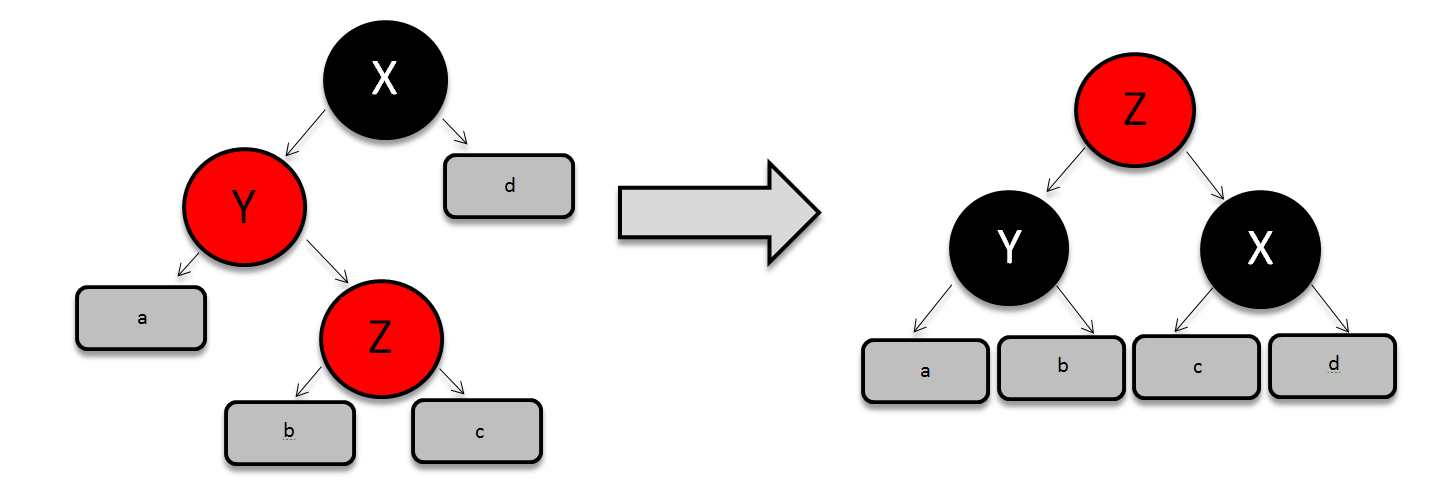
\includegraphics[width=\textwidth]{img/insert/clause_4.png}
				\caption{Случаи нарушения красно-черных свойств при вставке}
			\end{figure}
			
		
		\subsubsection{Удаление}
			Реализация использует арифметику цветов. К красному и черному цветам
			можно добавить или отнять черный цвет. Пусть при вычитании из красного цвета 
			черного цвета получится негативный черный, вычитание из черного цвета черного 
			даст красный цвет, добавление к красному цвету черного даст черный и добавление к
			черному цвету черного даст двойной черный цвет.
			\begin{figure}[H]
				\centering
				
\includegraphics[width=\textwidth]{img/tan-aus.png}
				\caption{Арифметика цветов}
			\end{figure}
			Реализуется арифметика цветов следующей функцией добавления цвета:
			\begin{lstlisting}
addBlack({Key, red, Left, Right}) ->
    {Key, black, Left, Right};
	
addBlack({Key, black, Left, Right}) ->
    {Key, doubleBlack, Left, Right}.			
			\end{lstlisting}
			Функция вычитания цвета не используется.
			
			Рассмотри алгоритм удаления. Для соблюдения красно-черных свойств необходимо:
			\begin{enumerate}
				\item Если у удаляемого узла 1 потомок и этот узел красный, то удаляем его, 
					  а на его место ставим единственного потомка.
					  Если у удаляемого узла 1 потомок и этот узел черный, то удаляем его,
					  а на его место ставим единственного потомка с увеличенным цветом.
					  Если у удаляемого узла 2 потомка, то удаляем его, а на его место 
					  ставим узел из левого поддерева с максимальным значением, удаляя 
					  из левого поддерева этот узел. 
				\item Произвести балансировку всего дерева, от корня к листьям, исправляя 
					  цвета узлов.
				\item Окрасить корень и листья в черный цвет, т.к. в процессе удаления 
					  и балансировки они могли изменить цвет. 
			\end{enumerate}
			
			\begin{lstlisting}
del_element(Key, Tree) -> 
    nilFix(make_black(del(Key, Tree))).
			\end{lstlisting}
			где 
			\begin{lstlisting}
nilFix({nil, doubleBlack, nil, nil}) ->
    {nil, black, nil, nil};
	
nilFix(Tree) ->
    Tree.					
			\end{lstlisting}	
			если агрументом является двойной черный лист преобразует его в черный,
			а если аргумент - дерево, то возвращает его без изменений.
			
			Рассмотрим функцию del, которая удаляет узел с заданным значением из дерева,
			а затем вызывает функцию балансировки дерева delFix. 
			\begin{lstlisting}
del(_, {nil, black, nil, nil}) ->
    {nil, black, nil, nil};
			\end{lstlisting}
			если производится попытка удалить узел из пустого дерева, то вернуть пустое дерево.
			\begin{lstlisting}
del(Key, {Key, red, Left, {nil, black, nil, nil}}) ->
    Left;
	
del(Key, {Key, red, {nil, black, nil, nil}, Right}) ->
    Right;
			\end{lstlisting}
			если цвет удаляемого узла красный, и у него есть только один потомок, то
			вернуть потомка.
			\begin{lstlisting}
del(Key, {Key, black, Left, {nil, black, nil, nil}}) ->
    addBlack(Left);
		
del(Key, {Key, black, {nil, black, nil, nil}, Right}) ->
    addBlack(Right);
			\end{lstlisting}
			если цвет удаляемого узла черный, и у него есть только один потомок, то
			вернуть потомка с добавленным цветом для сохранения 5 красно-черного свойства.
			\begin{lstlisting}
del(Key, {Key, Color, Left, Right})	->
    delFix({max(Left), Color, del(max(Left), Left), Right});
			\end{lstlisting}
			если у удаляемого узла 2 потомка, то вернуть дерево в котором вместо удаленного 
			узла будет узел с максимальным значением из его левого потомка, цвет удаленного узла, 
			левый потомок без своего максимального значения, а правый потомок останется без изменений.
			Результат необходимо сбалансировать.
			\begin{lstlisting}
del(Key, {KeyTree, ColorTree, LeftTree, RightTree}) 
    when Key < KeyTree ->
    delFix({KeyTree, ColorTree, del(Key, LeftTree), RightTree});
			
del(Key, {KeyTree, ColorTree, LeftTree, RightTree}) 
    when Key > KeyTree ->	
    delFix({KeyTree, ColorTree, LeftTree, del(Key, RightTree)}).
			\end{lstlisting}
			рекурсивный поиск удаляемого узла в дереве и балансировка дерева после 
			удаления.
			
			Функция delFix реализует следующие варианты нарушения красно-черных свойств 
			при удаалении узла:
			\begin{figure}[H]
				\centering
				
\includegraphics[width=\textwidth]{img/tan-aus.png}
				\caption{Cлучаи нарушения красно-черных свойств при удалении}
			\end{figure}
			
			
	\subsection{Логические функции}
		Для работы с упорядоченным множеством реализованы следующие логические операции:
		\begin{enumerate}
			\item Проверка на принадлежность элемента упорядоченному множеству
			\item Проверка на то, является ли одно упорядоченное множество
				  подмножеством другого
			\item Проверка на непересекаемость двух упорядоченных множеств
		\end{enumerate} 
		Рассмотрим каждую из них.
		
		\subsubsection{Принадлежность элемента множеству}
			Проверка на принадлежность элемента упорядоченному множеству
			реализуется с помощью функции is\_element(Elem, OSet), где Elem - 
			значение элемента, а OSet - упорядоченное множество.
			\begin{lstlisting}
is_element(_,  {nil, black, nil, nil}) ->
    false;				
			\end{lstlisting}
			Пустому множеству не может принадлежать никакой элемент.
			\begin{lstlisting}
is_element(Elem, {Elem, _, _, _}) ->
    true;
			\end{lstlisting}
			Если найден узел с искомым значением, то элемент принадлежит множеству.
			\begin{lstlisting}
is_element(Elem, {CurrElem, _, Left, Right}) ->		
    if
        Elem < CurrElem -> 
            is_element(Elem, Left);
        Elem > CurrElem -> 
            is_element(Elem, Right)
    end.	
			\end{lstlisting}
			Поиск элемента в дереве реализующем упорядоченное множество.
			
		\subsubsection{Является ли одно упорядоченное множество подмножеством другого}
			Проверка на то, является ли одно упорядоченное множество подмножеством другого
			реализуется с помощью функции is\_subset(OSetA, OSetB), где OSetA - предполагаемое
			подмножество OSetB.
			\begin{lstlisting}
is_subset({nil, black, nil, nil}, _) ->
    true;	
			\end{lstlisting}
			Пустое множество является подмножеством любого множества.	
			\begin{lstlisting}
is_subset({Key, _, Left, Right}, OSetB) ->
    IsElem = is_element(Key, OSetB),
    if
        IsElem -> 
            is_subset(Left, OSetB) 
            and 
            is_subset(Right, OSetB);
        true -> 
            false
    end.
			\end{lstlisting}
			Проверяется принадлежность корня OSetA множеству OSetB, и если корень
			принадлежит OSetB, то проверяется принадлежность левого и правого поддерева
			множеству OSetB. Иначе OSetA не является подмножеством OSetB.
			
		\subsubsection{Непересекаемость двух упорядоченных множеств}
			Проверка на непересекаемость двух упорядоченных множеств реализуется с помощью функции
			is\_disjoint(OSetA, OSetB), где OSetA и OSetB - упорядоченные множества.
			\begin{lstlisting}
is_disjoint(_, {nil, black, nil, nil}) ->
    true;	
			\end{lstlisting}
			Никакое множество не пересекается с пустым.
			\begin{lstlisting}
is_disjoint(OSetA, {Key, _, Left, Right}) ->
    IsElem = is_element(Key, OSetA),
    if
        IsElem -> 
            false;
        true -> 
            is_disjoint(OSetA, Left) 
            and 
            is_disjoint(OSetA, Right)
	end.
			\end{lstlisting}
			Проверяется принадлежность корня OSetB множеству OSetA, и если корень
			принадлежит OSetA, то множества не являются пересекающимися. Иначе
			проверяется непересекаемость левого и правого поддерева множеству OSetA.
		
		
	\subsection{Перевод в список и обратно, свертка и фильтрация}
		\subsubsection{Перевод упорядоченного множества в список}
			\begin{lstlisting}
to_list({nil, black, nil, nil}) ->
    [];
			\end{lstlisting}
			Пустое множество переводится в пустой список.
			\begin{lstlisting}
to_list({Key, _, Left, Right}) ->
    to_list(Left) ++ [Key] ++ to_list(Right).
			\end{lstlisting}
			Для сохранения упорядоченности в список переводится левое поддерево, потом 
			добавляется корневое значение, а затем в список переводится правое поддерево.
			
		\subsubsection{Перевод списка в упорядоченное множество}
			\begin{lstlisting}
from_list(List) ->
    lists:foldl(fun(Elem, OSet) -> 
                    add_element(Elem, OSet) 
                end, 
                new(), 
                List).
			\end{lstlisting}			
			Перевод списка в упорядоченное множество реализуется с помощью стандартной 
			функции свертки списка и функции добавления элемета в множество. К каждому 
			элементу списка List, применяется функция fun(Elem, OSet) где Elem - элемент
			List, а в качестве OSet изначально берется пустое множество.
			
		\subsubsection{Свертка}
			Свертка fold(Fun, Acc, OSet) применяет к каждому элементу упорядоченного
			множества OSet функцию Fun(Elem, Acc) и возвращает итоговое значение Acc.
			\begin{lstlisting}
fold(_, Acc, {nil, black, nil, nil}) ->
    Acc;	
			\end{lstlisting}
			Если свертка применяется к пустому множеству, то просто возвращается Acc.
			\begin{lstlisting}
fold(Fun, Acc, {Key, _, Left, Right}) ->
    Fun(Fun(Key, fold(Fun, Acc, Left)), fold(Fun, Acc, Right)).
			\end{lstlisting}
			Если же свертка применяется к не пустому множеству, то Fun применяется к левому, 
			а затем и к правому поддереву.
		
		\subsubsection{Фильтрация}
			Фильтрация filter(Pred, OSet) применяет к каждому элементу OSet предикат Pred, и 
			возвращает упорядоченное множество элементов из OSet удовлетворяющих Pred.
			\begin{lstlisting}
filter(Pred, OSet) ->
    OSetList = to_list(OSet),
    FilteredList = lists:filter(Pred, OSetList),
    from_list(FilteredList).	
			\end{lstlisting}
			Упорядоченное множество переводится в список, список фильтруется с помощью стандартной 
			функции, а затем результат переводится из списка обратно в упорядоченное множество.
			
			
	\subsection{Объединение, пересечение, разность}
		Реализации операций объединения, пересечения и разности отличаются друг от друга, для 
		достижения лучшей скорости.
		
		\subsubsection{Объединение}
			Операция объединения реализована рекурсивно. 
			\begin{lstlisting}			
union(OSetA, {nil, black, nil, nil}) ->
    OSetA;
			\end{lstlisting}
			Объединением упорядоченного множества OSetA с пустым, будет упорядоченное множество OSetA.
			\begin{lstlisting}
union(OSetA, {Key, _, Left, Right}) ->
    union(union(add_element(Key, OSetA), Left), Right).
			\end{lstlisting}
			Для объединения упорядоченных множеств OSetA и OSetB, во множество OSetA добавляется корневой 
			элемент OSetB, а после применяется операция объединения OSetA к левому и правому поддереву OSetB.  
		
			Для объединения более чем двух упорядоченных множеств используется функция объединения от списка
			упорядоченных множеств.
			\begin{lstlisting}
union([OSet1, OSet2 | []]) ->
    union(OSet1, OSet2);
			\end{lstlisting}
			Если в списке всего два упорядоченных множества, то использовать операцию объединения от двух 
			упорядоченных множеств.
			\begin{lstlisting}
union([OSet1, OSet2 | OSetsListTail]) ->
    OSetUnion = union(OSet1, OSet2),
    union([OSetUnion | OSetsListTail]).
			\end{lstlisting}
			В противном случае, заменить в исходном списке два первых упорядоченных множества
			их объединением и найти объединение нового списка.
				
		\subsubsection{Пересечение}
			Операция пересечения реализована перебором одного из упорядоченных множеств.
			\begin{lstlisting}
intersection(OSetA, OSetB) ->
    intersection(OSetA, OSetB, {nil, black, nil, nil}).
			\end{lstlisting}
			При первом вызове операции пересечения для упорядоченных множеств OSetA и OSetB
			вызывается функция пересечения с пустым аккумулятором.
			\begin{lstlisting}	
intersection({nil, black, nil, nil}, _, Acc) ->
    Acc;
			\end{lstlisting}
			При пересечении любого упорядоченного множества с пустым множеством необходимо вернуть аккумулятор.
			\begin{lstlisting}	
intersection(OSetA, OSetB, Acc) ->
    OSetALeft = min(OSetA),
    OSetANew = del_element(OSetALeft, OSetA),
    IsElem = is_element(OSetALeft, OSetB),
    if 
        IsElem =:= true -> 
            AccNew = add_element(OSetALeft, Acc),
            intersection(OSetANew, OSetB, AccNew);
        IsElem =:= false -> 
            intersection(OSetANew, OSetB, Acc)
    end.
			\end{lstlisting}
			В противном случае удаляем из упорядоченного множества OSetA минимальный элемент, и если он 
			принадлежит еще и множеству OSetB, то добавляем его в аккумулятор, иначе находим пересечение 
			нового упорядоченного множества OSetA и неизмененного OSetB.
			
			Функция пересечения более чем двух упорядоченных множеств реализуется аналогично с объединением:
			\begin{lstlisting}
intersection([OSet1, OSet2 | []]) ->
    intersection(OSet1, OSet2);

intersection([OSet1, OSet2 | OSetsListTail]) ->
    OSetIntersection = intersection(OSet1, OSet2),
    intersection([OSetIntersection | OSetsListTail]).
			\end{lstlisting}
			
		\subsubsection{Разность}
			Операция разности двух упорядоченных множеств, как и операция пересечения, реализована 
			перебором одного из упорядоченных множеств.
			\begin{lstlisting}
subtract(OSetA, {nil, black, nil, nil}) ->
    OSetA;
			\end{lstlisting}
			Вычитание из упорядоченного множества OSetA пустого множества даст упорядоченное множество OSetA.
			\begin{lstlisting}
subtract(OSetA, OSetB) ->
    OSetBLeft = min(OSetB),
    OSetBNew = del_element(OSetBLeft, OSetB),
    IsElem = is_element(OSetBLeft, OSetA),
    if 
        IsElem =:= true -> 
            OSetANew = del_element(OSetBLeft, OSetA),
            subtract(OSetANew, OSetBNew);
        IsElem =:= false -> 
            subtract(OSetA, OSetBNew)
    end.	 	
			\end{lstlisting}
			Если же из упорядоченного множества OSetA вычитаем непустое упорядоченное множество OSetB,
			то удаляем из упорядоченного множества OSetB минимальный элемент, и если он 
			принадлежит еще и множеству OSetA, то удаляем его из множества OSetA и вычитаем из нового
			упорядоченного множества OSetA новое упорядоченное множество OSetB, иначе вычитаем из неизмененного
			упорядоченного множества OSetA новое упорядоченное множество OSetB.
			
			
			
			
\section{Сравнение с модулями sets и ordsets}
	В своей работе я произвел сравнение времени выполнения стандартных операций реализованной мной структуры, со 
	стандарными структурами языка Erlang. Свою реализацию упорядоченного множества oset я сравниваю со стандарным 
	упорядоченным множеством ordsets, и	стандартным множеством sets.
	
	В ходе сравнения данные считывались из текстового файла, заносились в структуру и для каждой структуры проводились
	замеры времени выполнения ее функций. Замер происходил дважды. В первый раз в текстовом файле находилось 100 000 чисел 
	от 0 до 2 147 483 647 и 99 997 уникальных значений, а во второй от 0 до 10 000 и 10 000 уникальных значений. Время 
	указано в секундах.
	
	\subsection{Вставка и удаление}
		В приведенных ниже временных показателях указано среднее время считывания 100 000 чисел из файла и занесения 
		их в структуру.
		
		\begin{figure}[H]
				\centering
				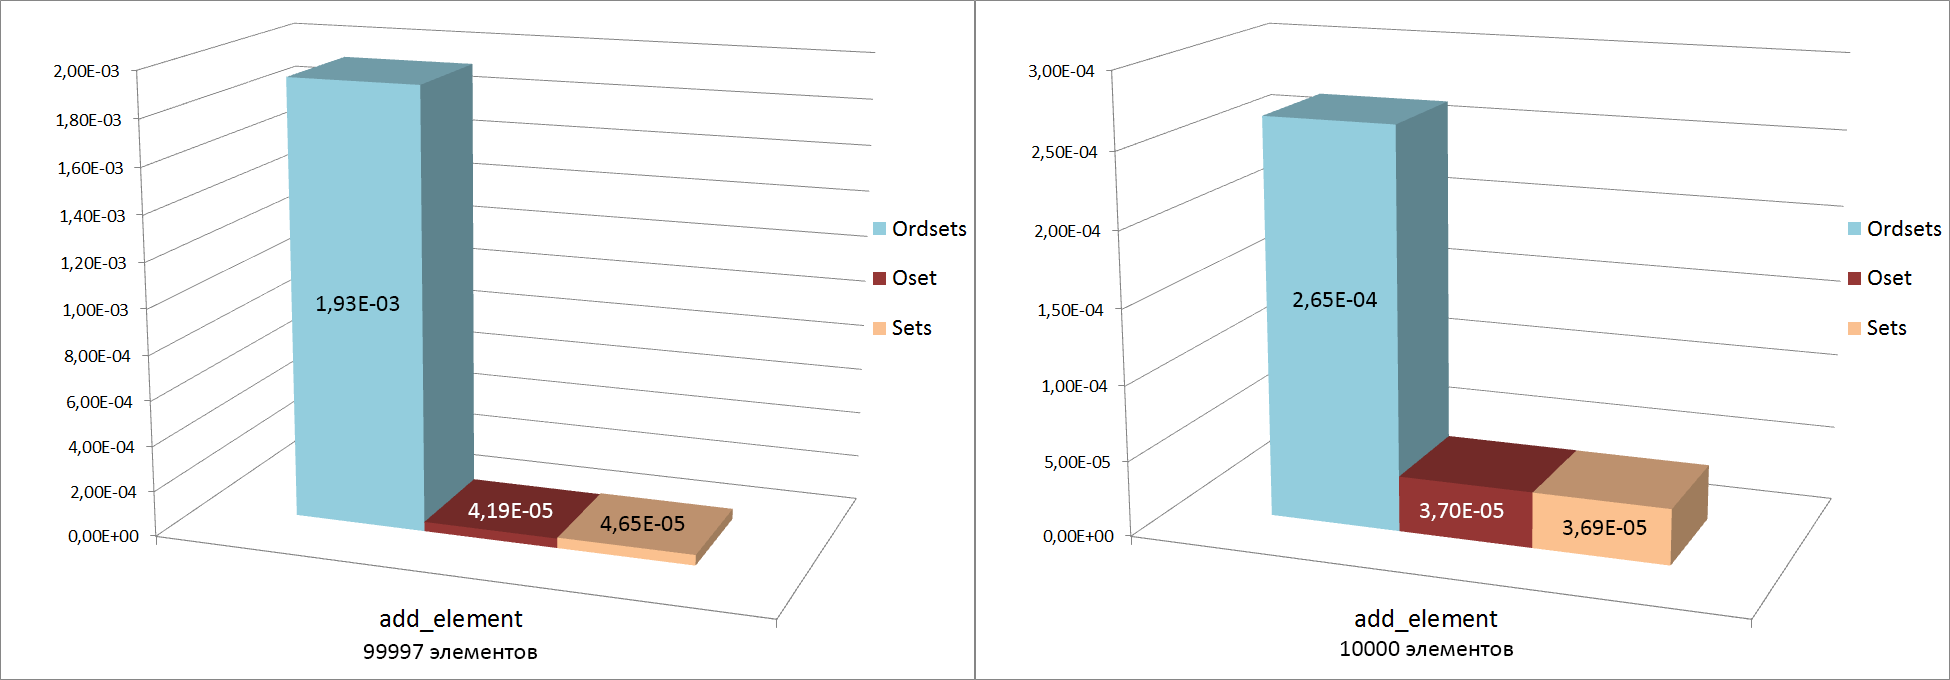
\includegraphics[width=\textwidth]{img/histograms/add_element.png}
				\caption{Замер времени выполнения операции вставки}
		\end{figure}
		
		Аналогично и для операции удаления - время считывания чисел из файла и удаление их из структуры. 
		
		\begin{figure}[H]
				\centering
				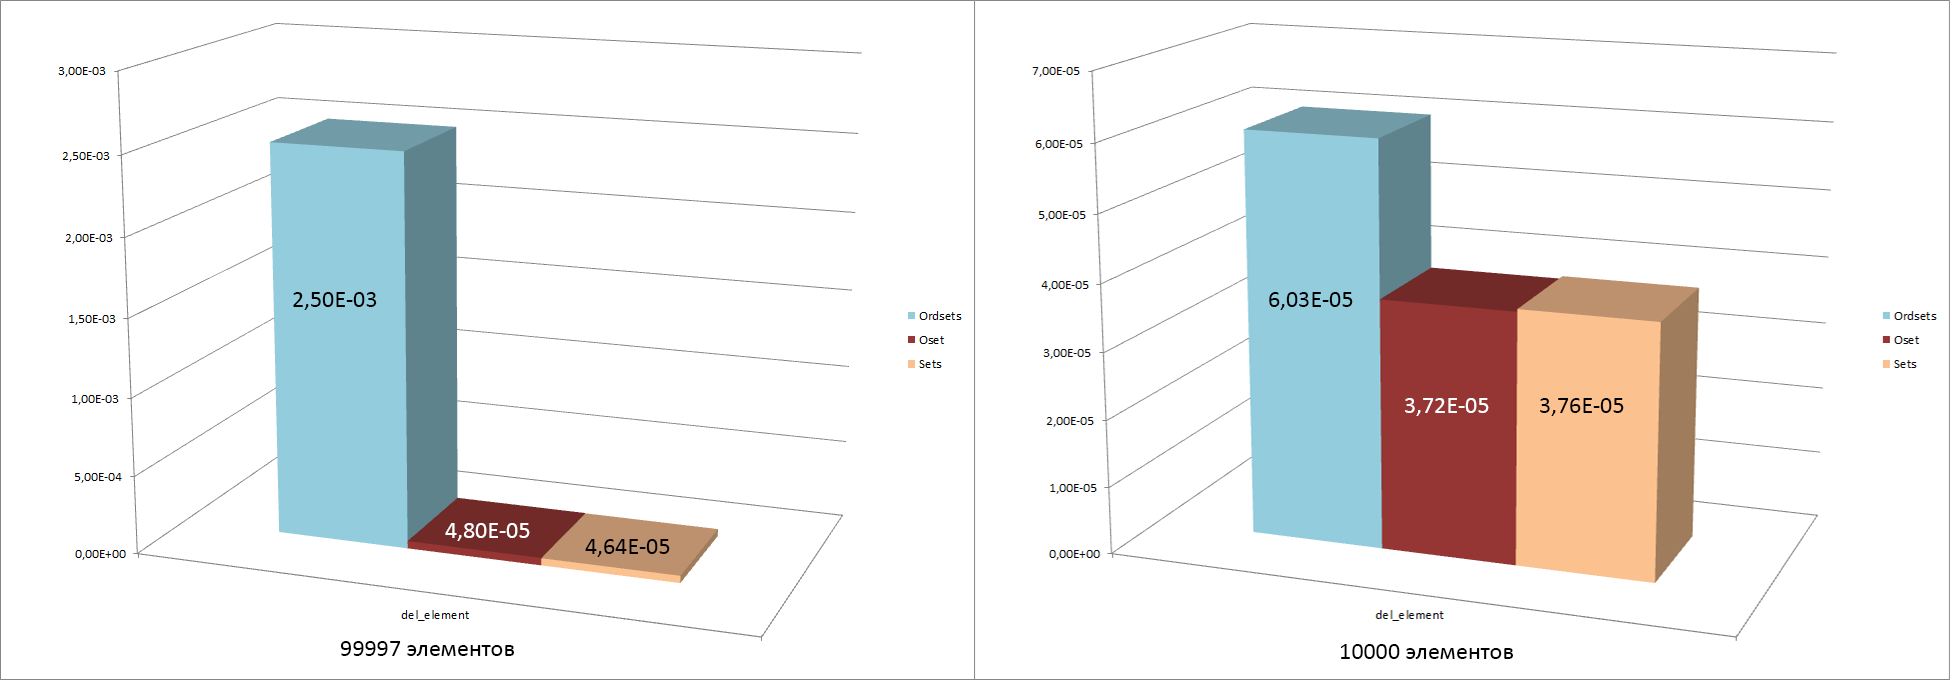
\includegraphics[width=\textwidth]{img/histograms/del_element.png}
				\caption{Замер времени выполнения операции удаления}
		\end{figure}
		
		Как видно из рисунков 16 и 17, время выполнения операций вставки и удаления из модуля oset, сопоставимо 
		с временем выполнения операций в модуле sets, и существенно меньше времени выполнения этих операций
		в модуле ordsets. Это связано с тем, что упорядоченное множество в модуле ordsets реализовано 
		списком Erlang, а операции вставки и удаления линейны. 	
		
	\subsection{Логические функции}
		Логические функции, такие как is\_element, is\_subset и is\_disjoint запускаются по 100 раз
		каждая и в результат идет среднее время выполнения.
		
		\begin{figure}[H]
				\centering
				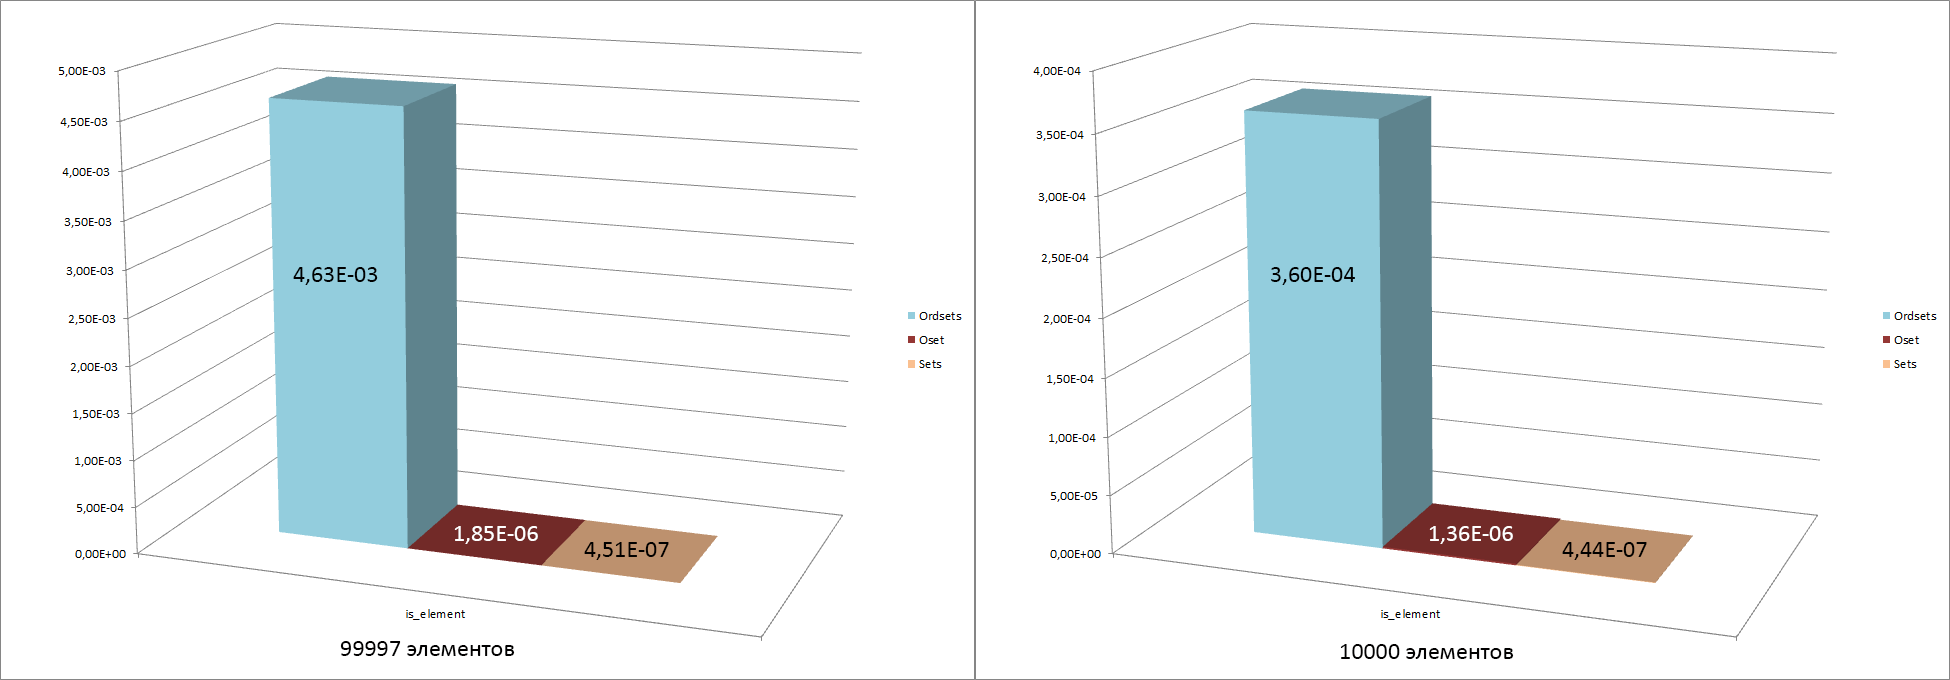
\includegraphics[width=\textwidth]{img/histograms/is_element.png}
				\caption{Замер времени выполнения проверки на принадлежность элемента множеству}
		\end{figure}
		Благодаря тому, что модуль oset реализует упорядоченное множество на основе красно-черного дерева, операция
		проверки на принадлежность элемента множеству работает примерно за то же время, что и у модуля sets, и на 
		несколько порядков быстрее, чем у модуля ordsets, так как в нем эта операция реализована перебором всех элементов
		списка.  
		
		\begin{figure}[H]
				\centering
				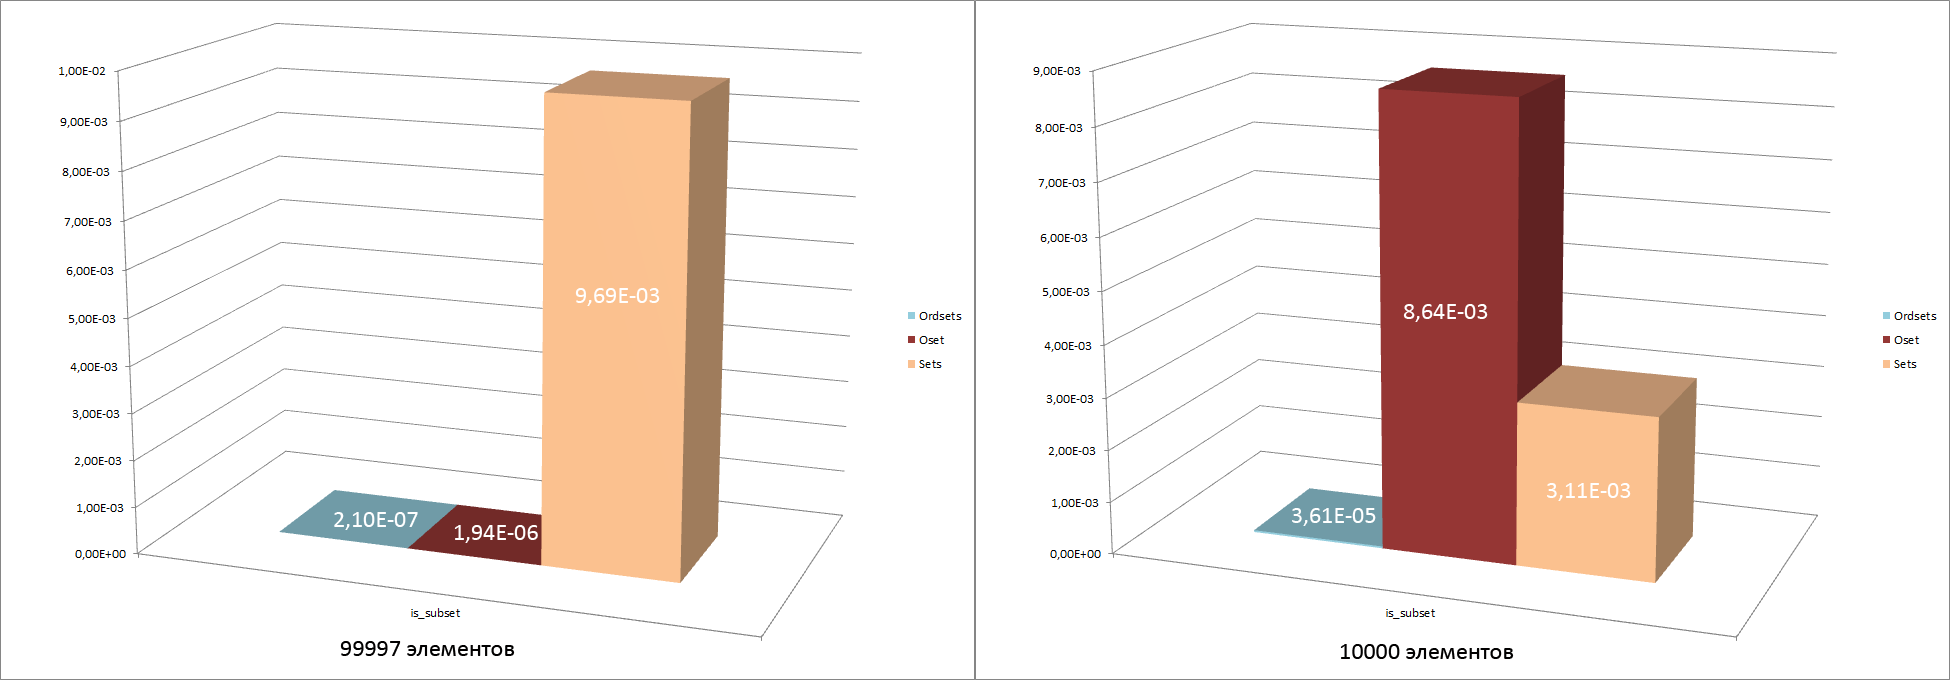
\includegraphics[width=\textwidth]{img/histograms/is_subset.png}
				\caption{Замер времени выполнения проверки на то, является ли одно множество подмножеством другого}
		\end{figure}
		При большом объеме данных множества реализация проверки в модуле sets заметно уступает по времени 
		выполнения модулям ordsets и sets. Это связано с тем, что в модуле sets проверка реализована 
		последовательным перебором элементов одного множества и проверкой на его принадлежность другому. При малом 
		объеме данных реализация в модуле ordsets работает быстрее, из-за реализации струтуры данных с помощью 
		списка Erlang.  
		
		\begin{figure}[H]
				\centering
				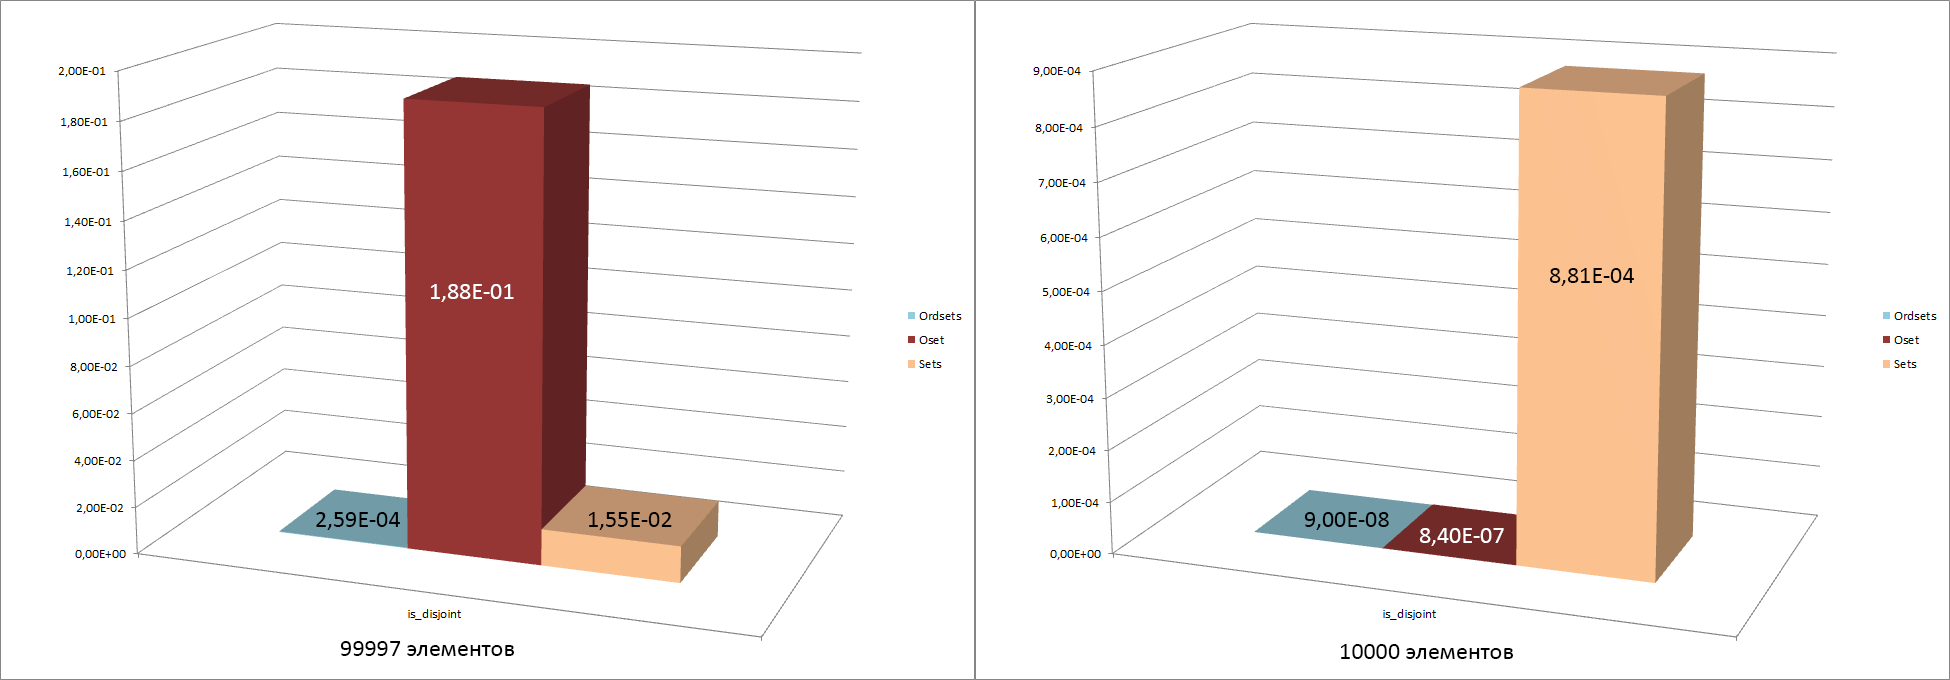
\includegraphics[width=\textwidth]{img/histograms/is_disjoint.png}
				\caption{Замер времени выполнения проверки на непересекаемость двух упорядоченных множеств}
		\end{figure}
		Реализация данной проверки в модуле sets при малом количестве данных работает медленнее, как и в случае 
		с проверкой на то, является ли одно множество подмножеством другого, из-за последовательного перебора 
		элементов одного множества. При большом объеме данных рекурсивная реализация oset, уступает реализациям из 
		модулей ordsets и sets.
				
	
	\subsection{Перевод в список и обратно, свертка и фильтрация}
		При замере времени, как и с логическими функциями, каждая функция запускается по 100 раз, а в результат идет 
		среднее время выполнения.
		
		\begin{figure}[H]
				\centering
				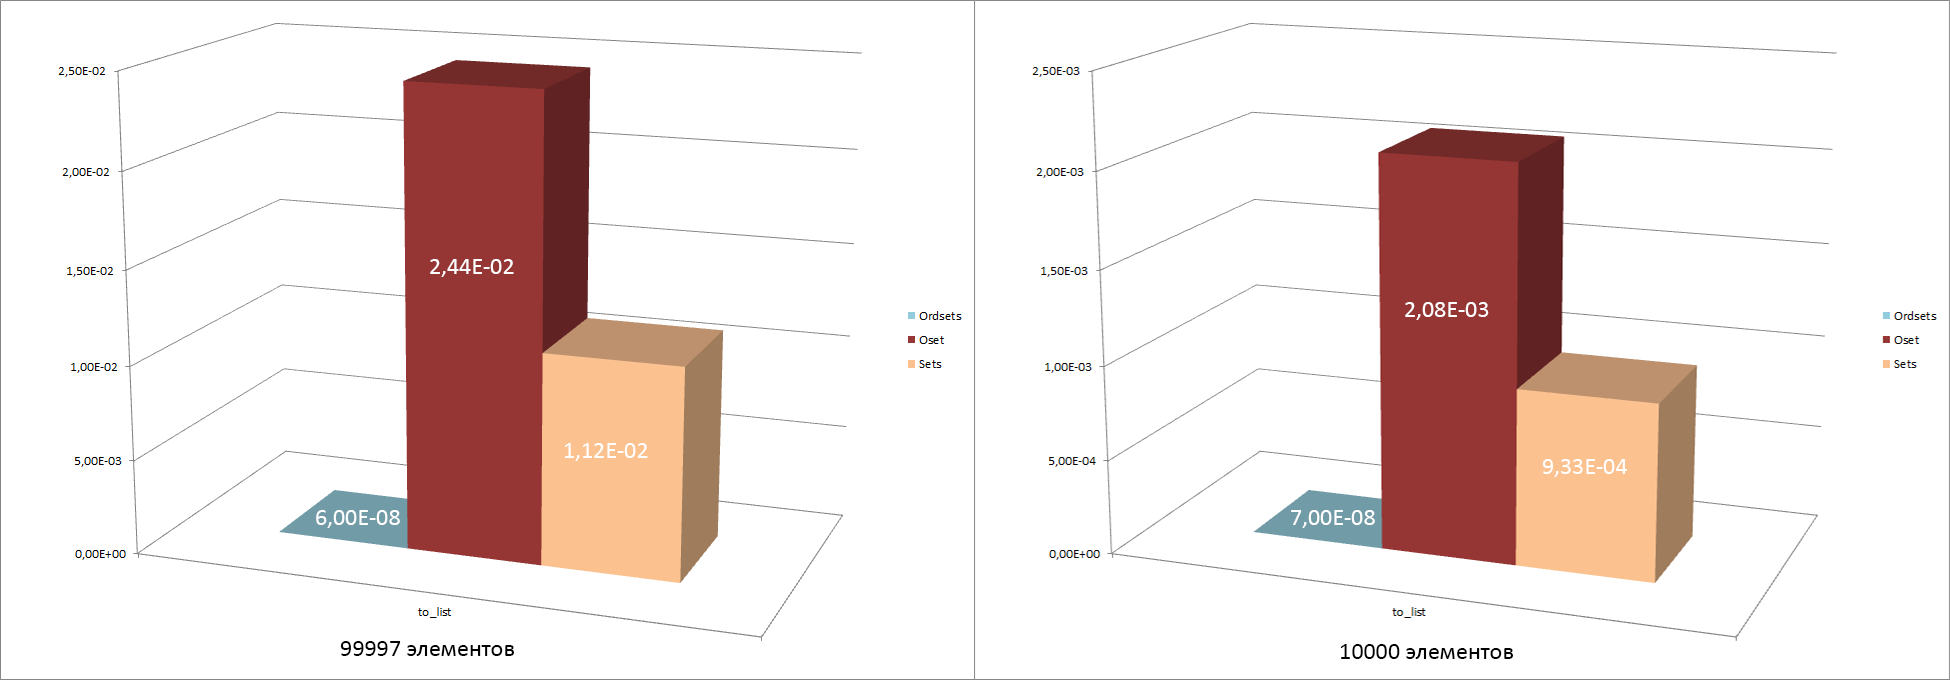
\includegraphics[width=\textwidth]{img/histograms/to_list.png}
				\caption{Замер времени выполнения перевода множества в список}
		\end{figure}
		Самой быстрой операцией перевода множества в список является реализация из модуля ordsets, так как 
		само множество реализовано с помощью списка. Реализация модуля sets использует операцию свертки и 
		поэлементно заполняет список. Реализация модуля oset рекурсивно добаляет в список значение корня,
		и добавляет к нему в начало список из левого поддерева, а в конец - из правого.
		
		\begin{figure}[H]
				\centering
				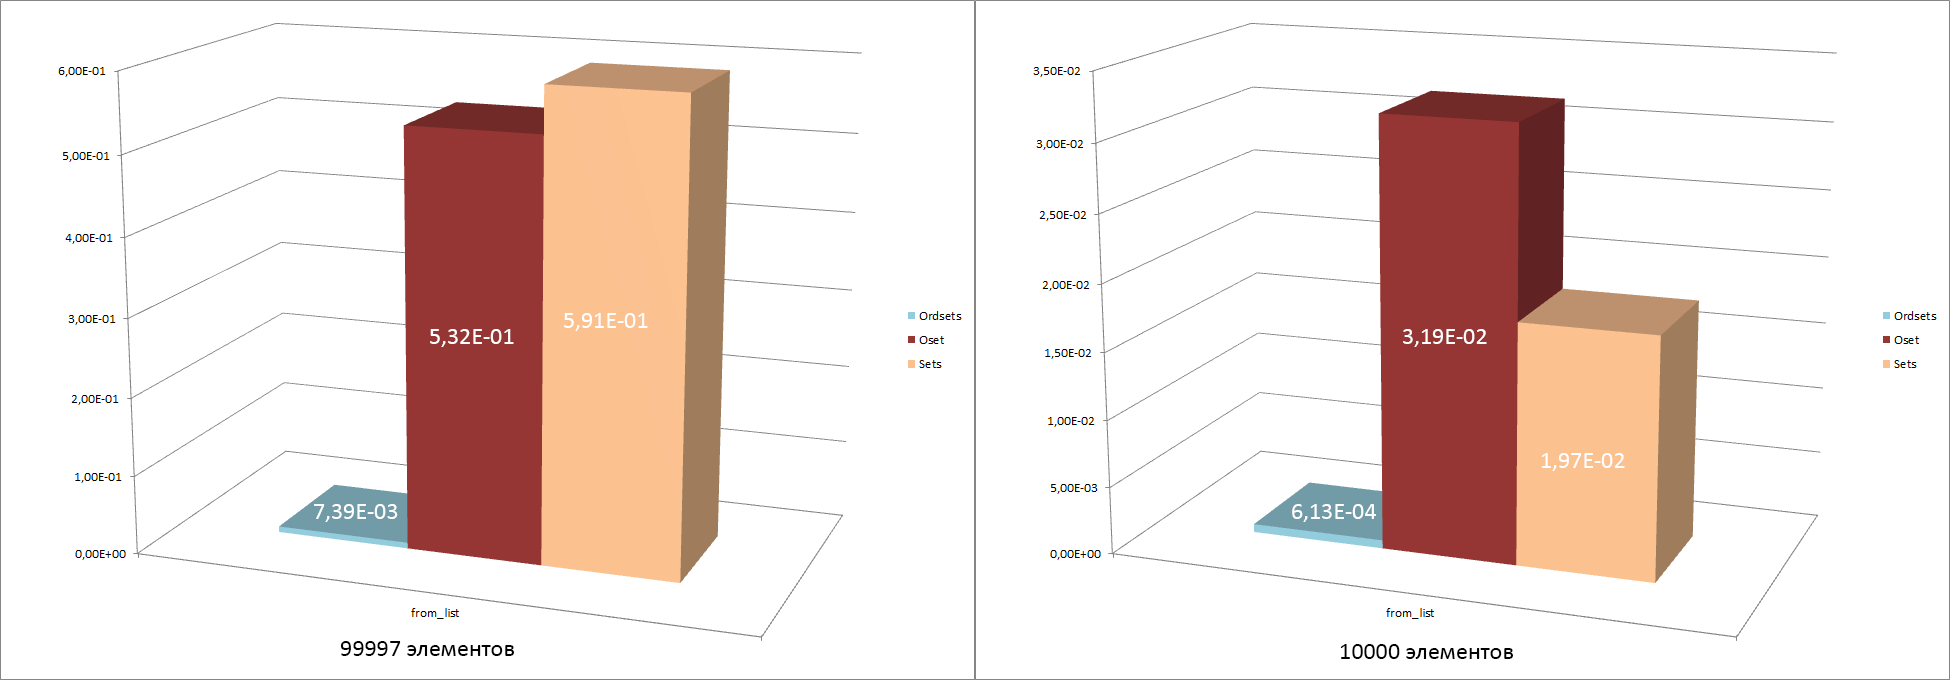
\includegraphics[width=\textwidth]{img/histograms/from_list.png}
				\caption{Замер времени выполнения перевода списка в множество}
		\end{figure}
		На большом объеме множества реализации из модулей oset и sets работают приблизительно одинакого.
		Реализация модуля ordsets работает быстрее, так как она просто сортирует список.
		На малом объеме данных реализация модуля oset уступает реализации модeля sets.
		
		\begin{figure}[H]
				\centering
				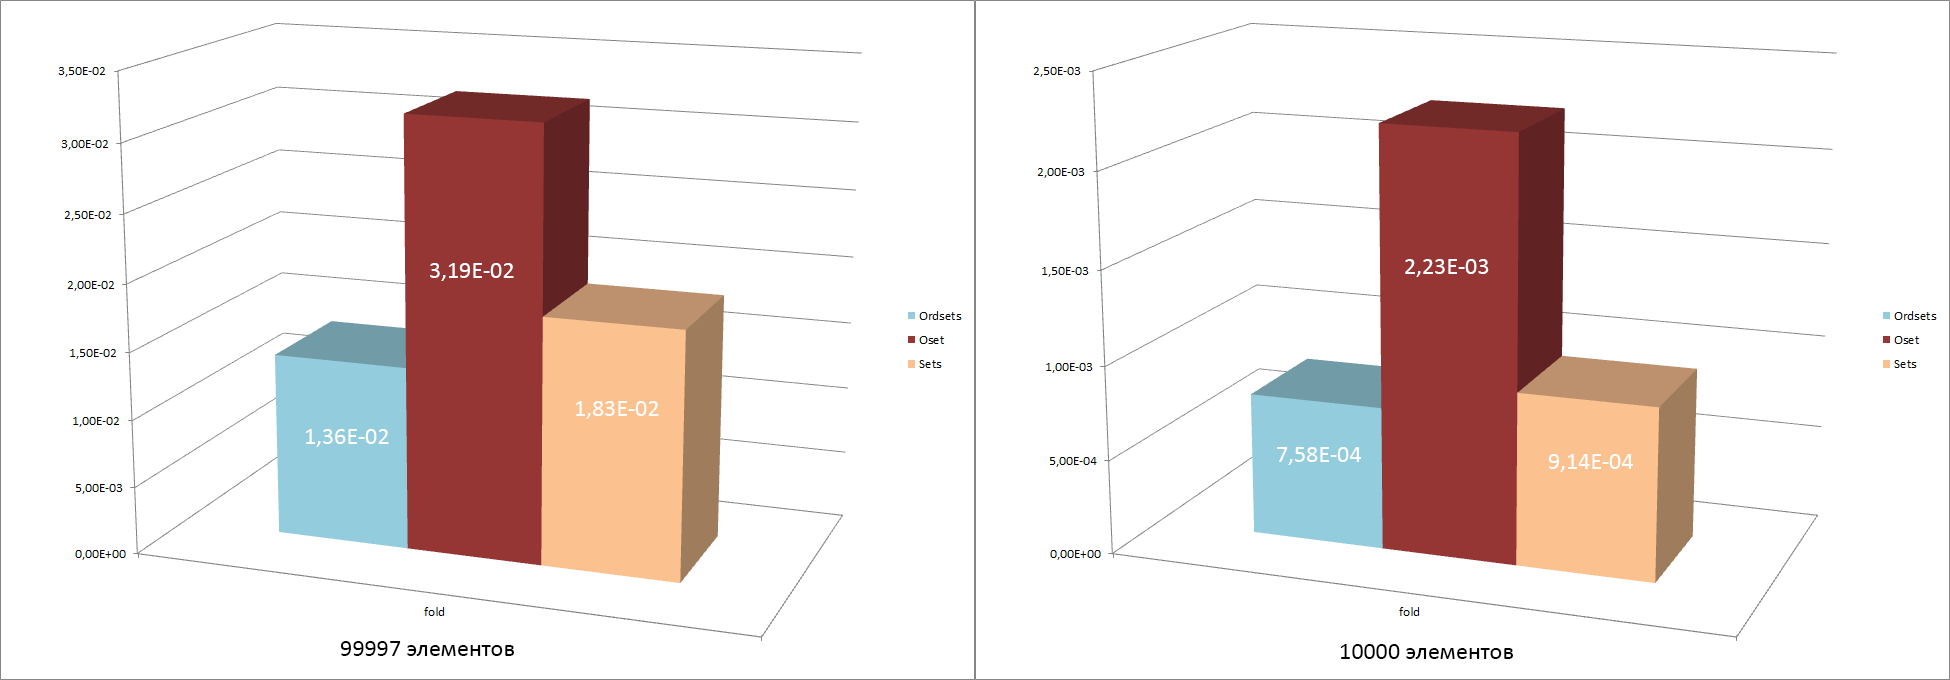
\includegraphics[width=\textwidth]{img/histograms/fold.png}
				\caption{Замер времени выполнения свертки}
		\end{figure}
		Свертка проверялась на функции сложения. Резултатом ее выполнения являлась сумма элементов множества.
		Erlang умеет работать с большими числами, поэтому ошибок при вычислении свертки не происходило.
		Показатели времени выполнения операции свертки не сильно отличаются друг от друга, несмотря на то, что
		свертка в модуле ordsets реализована стандартной операцией свертки над списком. 

		\begin{figure}[H]
				\centering
				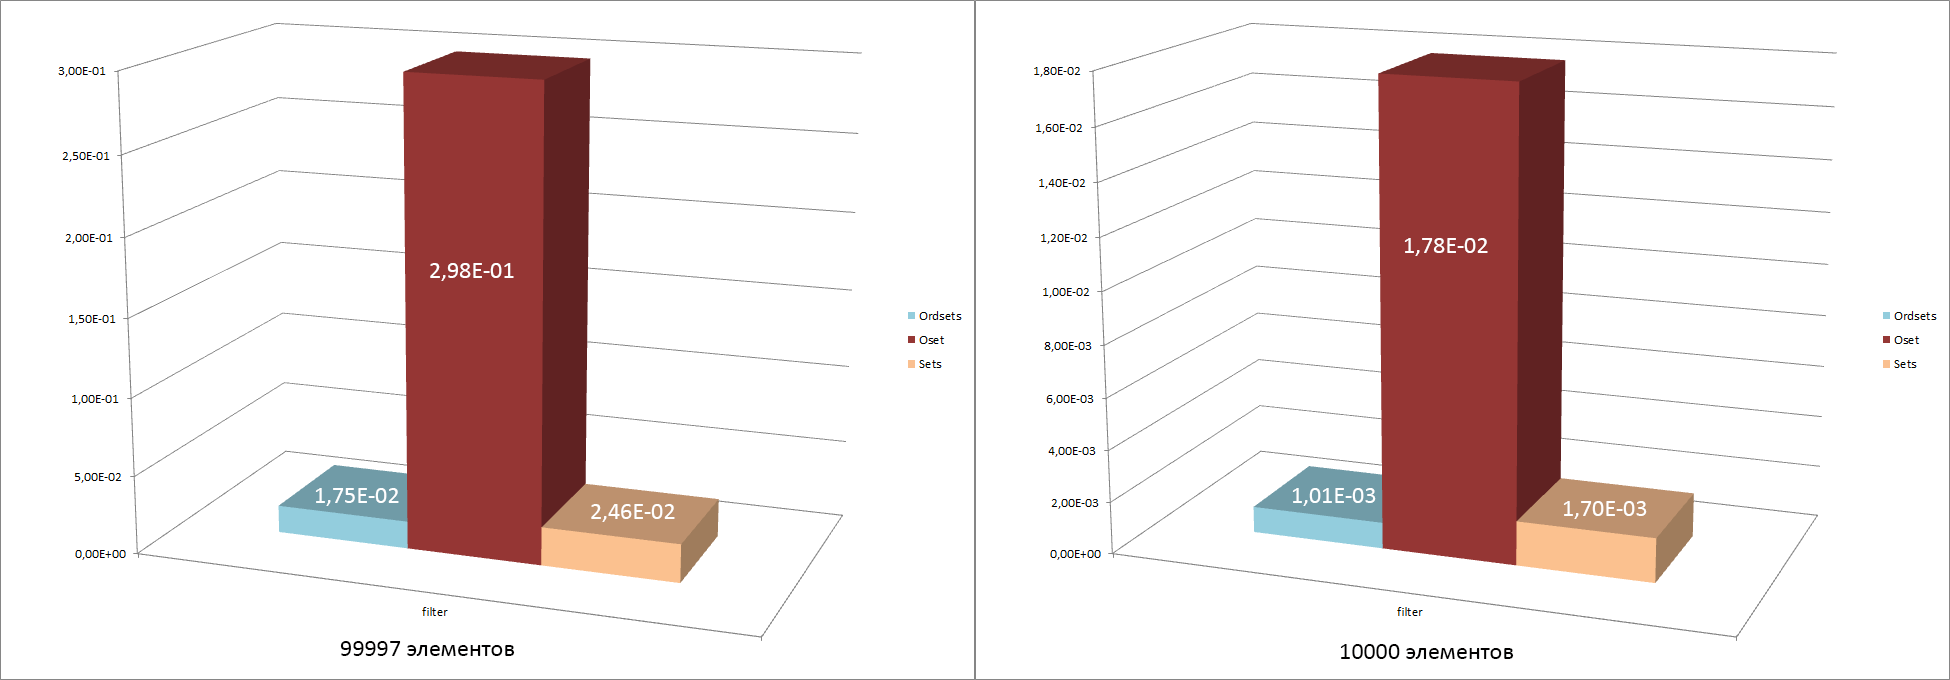
\includegraphics[width=\textwidth]{img/histograms/filter.png}
				\caption{Замер времени выполнения фильтрации}
		\end{figure}
		Фильтрация проверялась на предикате проверяющем четность числа. Результатом ее выполнения являлось множество
		четных элементов. Операция фильтрации множества в модуле oset по времени выполнения уступает реализациям 
		модулей sets и ordsets. Отставание по времени связано с тем, что реализация oset использует перевод множества в 
		список и стандартную реализацию операции фильтрации для списка.

	\subsection{Объединение, пересечение, разность}
		Операции объединения, пересечения и разности запускаются по 100 раз и в результат 
		идет среднее время выполнения.
		
		\begin{figure}[H]
				\centering
				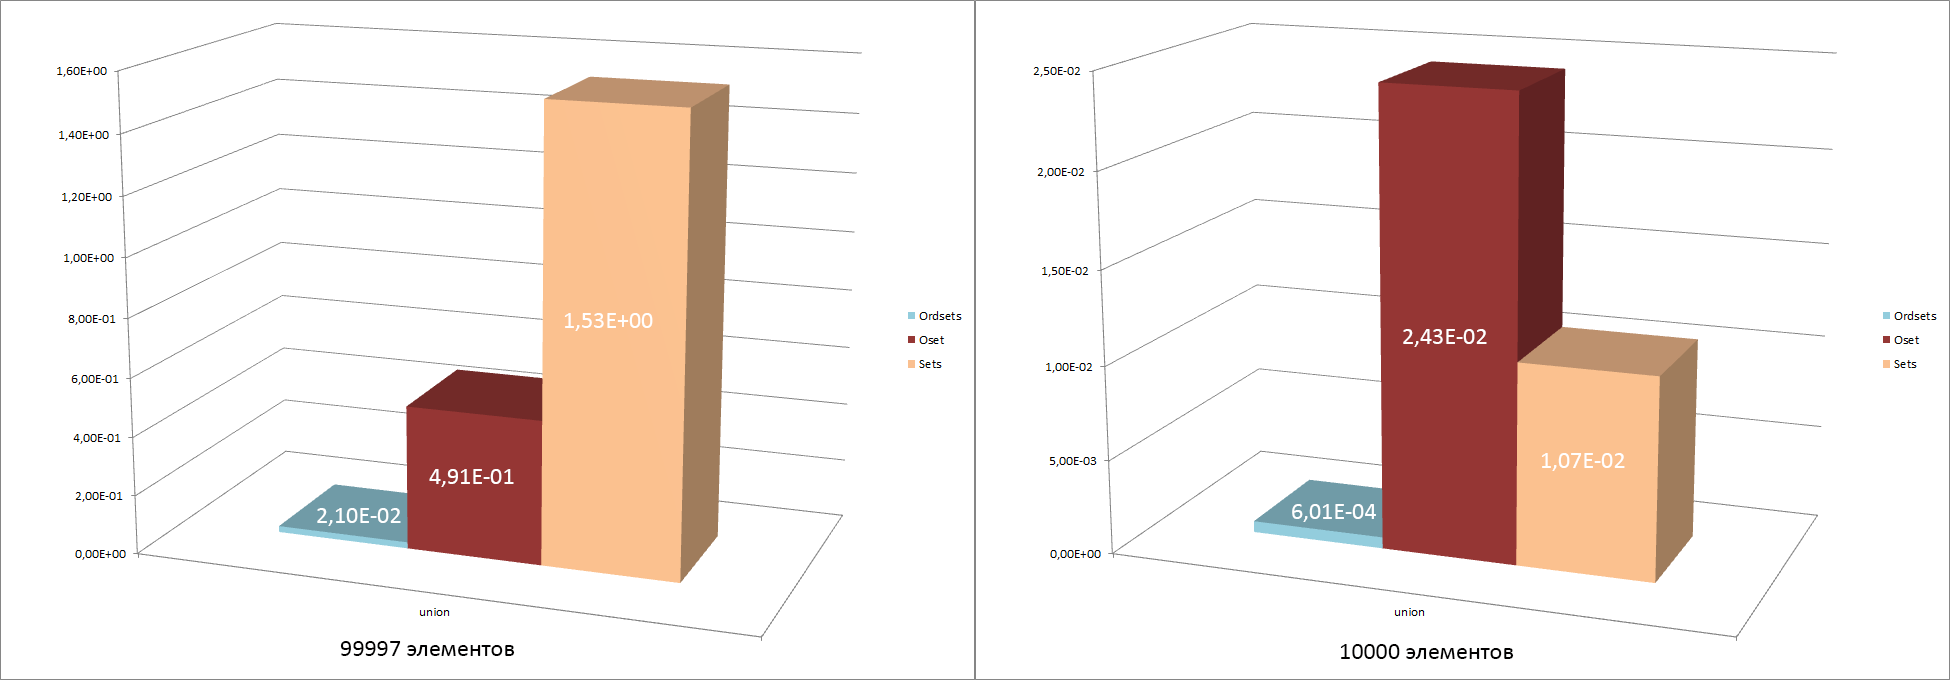
\includegraphics[width=\textwidth]{img/histograms/union.png}
				\caption{Замер времени выполнения объединеия двух множеств}
		\end{figure}
		На большом объеме данных реализация модуля sets уступает двум другим, потому что реализована с поможщью свертки.
		На малом объеме данных в модуле oset самая медленная реализация операции объединения двух множеств, так как
		реализована рекурсивно. Реализация модуля ordsets в обоих случаях работает быстрее. Это происходит из-за 
		реализации самого множества с помощью списка, и быстроты операций с ним.
		
		\begin{figure}[H]
				\centering
				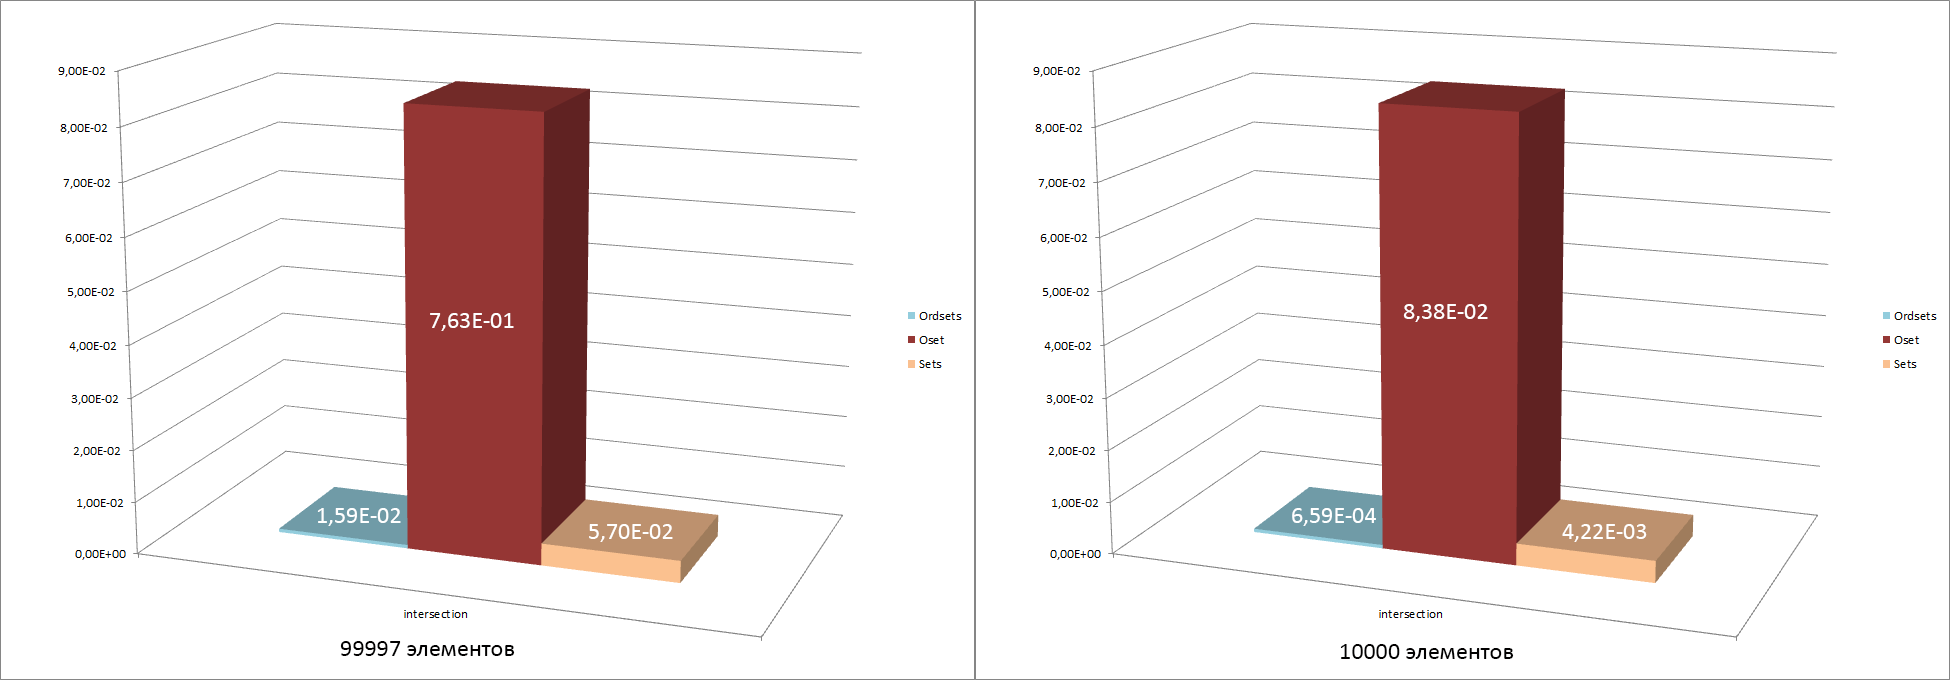
\includegraphics[width=\textwidth]{img/histograms/intersection.png}
				\caption{Замер времени выполнения пересечения двух множеств}
		\end{figure}
		
		\begin{figure}[H]
				\centering
				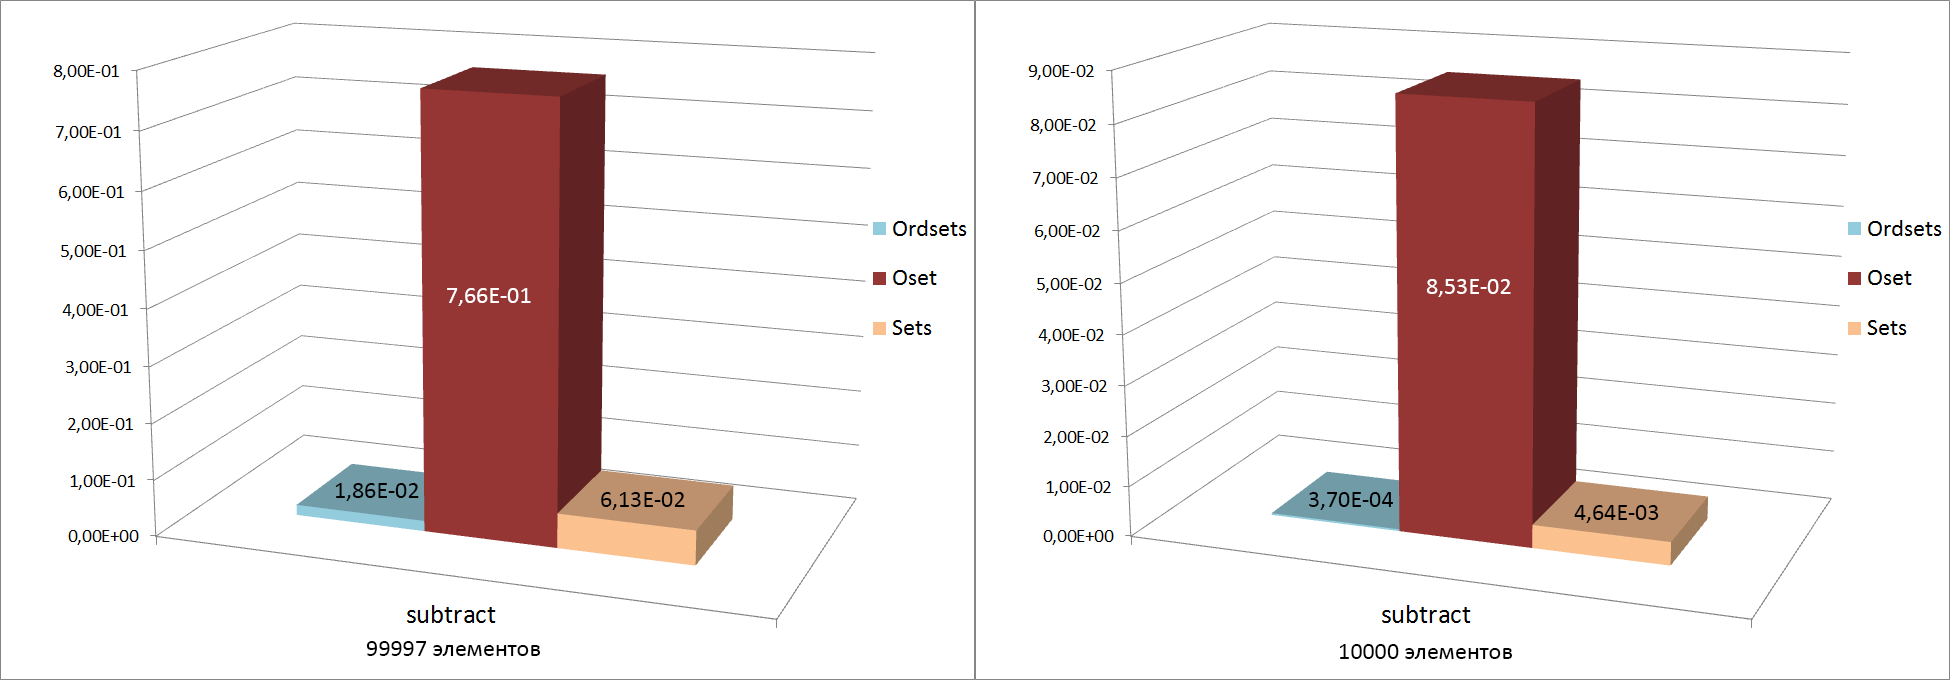
\includegraphics[width=\textwidth]{img/histograms/subtract.png}
				\caption{Замер времени выполнения разности двух множеств}
		\end{figure}
		Время выполнения операций пересечения двух упорядоченных множеств и их разности в модуле oset уступает времени
		выполнения этой	же операции в модулях sets и ordsets. Длительность выполнения связана с последовательным перебором
		всех элементов одного из множеств.
		

\section{Несколько примеров в~\LaTeX{}}
\label{sec:examples}

Некоторые часто используемые
команды приведены в качестве примера ниже (и варианты — в
комментариях). Мы рекомендуем внимательно прочесть данный
текст и изучить его исходный код прежде, чем начинать писать
свой собственный. Кроме того, можно дать и такой совет: идущий
ниже текст не убирать до самого конца, а просто оставлять его
позади своего собственного текста, чтобы в любой момент можно
было проконсультироваться с данными примерами.

\subsection{Как вставлять листинги и рисунки}

Для крупных листингов есть два способа. Первый красивый, но в нём не допускается
кириллица (у вас может встречаться в комментариях и
печатаемых сообщениях), он представлен на листинге~\ref{list:hwbeauty}.
\begin{ListingEnv}[H]% буква H означает Here, ставим здесь,
% элементы, которые нежелательно разрывать обычно не ставят
% посреди страницы: вместо H используется t (top, сверху страницы),
% или b (bottom) или p (page, на отдельной странице)
\begin{lstlisting}
#include <iostream>
using namespace std;

int main()
{
    cout << "Hello, world" << endl;
    system("pause");
    return 0;
}
\end{lstlisting}
%следующую команду для генерации подписи можно опустить,
% хотя рекомендуется все специальные элементы (таблицы, рисунки,
% листинги) подписывать. Если подпись пропустить, листинг также не получит
% номера и на него не сошлёшься в будущем
\caption{Программа “Hello, world” на \protect\cpp}
% далее метка для ссылки:
\label{list:hwbeauty}
\end{ListingEnv}

Второй не такой красивый, но без ограничений (см.~листинг~\ref{list:hwplain}).
\begin{ListingEnv}[H]
\begin{Verb}

#include <iostream>
using namespace std;

int main()
{
    cout << "Привет, мир" << endl;
}
\end{Verb}
\caption{Программа “Hello, world” без подсветки}
\label{list:hwplain}
\end{ListingEnv}

Можно использовать первый для вставки небольших фрагментов
внутри текста, а второй для вставки полного
кода в приложении, если таковое имеется.

Если нужно вставить совсем короткий пример кода (одна или две строки), то выделение  линейками и нумерация может смотреться чересчур громоздко. В таких случаях можно использовать окружения \texttt{lstlisting} или \texttt{Verb} без \texttt{ListingEnv}. Приведём такой пример с указанием языка программирования, отличного от заданного по умолчанию:
\begin{lstlisting}[language=Haskell]
fibs = 0 : 1 : zipWith (+) fibs (tail fibs)
\end{lstlisting}
Такое решение~--- со вставкой нумерованных листингов покрупнее
и вставок без выделения для маленьких фрагментов~--- выбрано,
например, в книге Эндрю Таненбаума и Тодда Остина по архитектуре
компьютера~\autocite{TanAus2013} (см.~рис.~\ref{fig:tan-aus}).

Наконец, для оформления идентификаторов внутри строк
(функция \lstinline{main} и тому подобное) используется
\texttt{lstinline} или, самое простое, моноширинный текст
(\texttt{\textbackslash texttt}).

\begin{figure}[p]% p означает, что нужно выделить для рисунка
% отдельную страницу; применяется для больших рисунков
\centering
%Здесь могла быть ваша лягушка.

\includegraphics[width=\textwidth]{img/tan-aus.png}
\caption{\label{fig:tan-aus}Пример оформления листингов в~\autocite{TanAus2013}}
\end{figure}

Использовать внешние файлы (например, рисунки) можно и на \href{http://overleaf.com}{overleaf.com}: ищите кнопочку upload.

\subsection{Как оформить таблицу}

Для таблиц обычно используются окружения table и tabular --- см. таблицу~\ref{tab:widgets}. Внутри окружения tabular используются специальные команды пакета booktabs — они очень красивые; самое главное: использование вертикальных линеек считается моветоном.

\begin{table}
\centering
\caption{\label{tab:widgets}Подпись к таблице --- сверху}
\begin{tabular}{llr}
\toprule
\multicolumn{2}{c}{Item} \\
\cmidrule(r){1-2}
Животное  & Описание    & Цена (\$) \\
\midrule
Gnat      & per gram    & 13.65      \\
          & each        & 0.01       \\
Gnu       & stuffed     & 92.50      \\
Emu       & stuffed     & 33.33      \\
Armadillo & frozen      & 8.99       \\
\bottomrule
\end{tabular}
\end{table}

\subsection{Как набирать формулы}

\LaTeX{} is great at typesetting mathematics. Let $X_1, X_2, \ldots, X_n$ be a sequence of independent and identically distributed random variables with $\text{E}[X_i] = \mu$ and $\text{Var}[X_i] = \sigma^2 < \infty$, and let
$$S_n = \frac{X_1 + X_2 + \cdots + X_n}{n}
      = \frac{1}{n}\sum_{i}^{n} X_i$$
denote their mean. Then as $n$ approaches infinity, the random variables $\sqrt{n}(S_n - \mu)$ converge in distribution to a normal $\mathcal{N}(0, \sigma^2)$.

\subsection{Как оформлять списки}

Нумерованные списки (окружение enumerate, команды item)…

\begin{enumerate}
  \item Like this,
  \item and like this.
\end{enumerate}

\dots маркированные списки \dots

\begin{itemize}
  \item Like this,
  \item and like this.
\end{itemize}

\dots списки-описания \dots

\begin{description}
  \item[Word] Definition
  \item[Concept] Explanation
  \item[Idea] Text
\end{description}

\Conc

Помните, что на все пункты списка литературы должны быть ссылки. \LaTeX\ просто не добавит информацию об издании из bib"/файла, если на это издание нет ссылки в тексте. Часто студенты используют в работе  электронные ресурсы: в этом нет ничего зазорного при одном условии: при каждом заимствовании следует ставить соответствующую ссылку. В качестве примера приведём ссылку на сайт нашего института~\autocite{mmcs}.

Для дальнейшего изучения \LaTeX\ рекомендуем книгу Львовского~\autocite{Lvo2003}: она хорошо написана, хотя и несколько устарела.
Обычно стоит искать подсказки на
\href{http://tex.stackexchange.com/}{tex.stackexchange.com}, а также
читать документацию по установленным пакетам с помощью
команды
\begin{Verb}
texdoc имя_пакета
\end{Verb}
или на \href{http://ctan.org/}{ctan.org}.

% Печать списка литературы (библиографии)
\printbibliography[%{}
    heading=bibintoc%
    %,title=Библиография % если хочется это слово
]
% Файл со списком литературы: biblio.bib
% Подробно по оформлению библиографии:
% см. документацию к пакету biblatex-gost
% http://ctan.mirrorcatalogs.com/macros/latex/exptl/biblatex-contrib/biblatex-gost/doc/biblatex-gost.pdf
% и огромное количество примеров там же:
% http://mirror.macomnet.net/pub/CTAN/macros/latex/contrib/biblatex-contrib/biblatex-gost/doc/biblatex-gost-examples.pdf

\end{document}
